\chapter{Cryptic splicing occurs in published TDP-43 but not FUS depletion data}
\label{chapter:cryptic_exons}
%SORT OUT APPENDICES

This chapter has been published as \citep{Humphrey2017}. See appendices for full reproduction of the manuscript.

\section{Overview}

Ling and colleagues observed the inclusion of cryptic exons when TDP-43 was depleted in HeLa or mouse embryonic stem cells \citep{Ling2015}. These cryptic exons were shown to originate from poorly evolutionarily conserved sequence and shared no positions between the two species. These findings raise the possibility that impaired exon recognition contributes to TDP-43's role in ALS aetiology.

I aimed to replicate and expand the findings of Ling and colleagues. I first developed a quantitative genome-wide analysis pipeline to detect and classify cryptic splicing. I then applied this pipeline to seven datasets (four human and three murine models) to systematically quantify cryptic splicing alterations associated with depletion of TDP-43. In addition I investigated FUS in order to determine whether modulation of cryptic splicing was a common feature of RNA-binding proteins implicated in ALS. Furthermore I analysed hnRNP C, as it had been previously shown to repress cryptic exons originating from Alu repeat elements. Lastly, I used independent protein-RNA interaction datasets, conservation data, repeat element annotation and splice site scoring to investigate the potential mechanisms linking TDP-43 depletion with the cryptic exon phenomenon.





\section{Methods}

\subsection{Data preparation}
Table \ref{table:cryptic_data} lists all the public data used in this study. All RNA-seq data was downloaded in the FASTQ format and processed using our RNA-seq pipeline (see methods chapter).
Processed iCLIP peak data was downloaded from the iCOUNT server. Both the human and mouse TDP-43 iCLIP data have been previously published \citep{Tollervey2011,Rogelj2012}.

Processed eCLIP data (previously described by \citep{Van_Nostrand2016-su}) was downloaded from the ENCODE project. The narrowPeaks bed format was used with the first nucleotide of the cluster defined as the peak. Peak coordinates from iCLIP and eCLIP were converted to the hg38 and mm10 builds using the \emph{LiftOver} tool from UCSC. 

\begin{table}[h!]
	\caption[List of accessions]{
		\textbf{List of accessions}
	}
	\label{table:cryptic_data}
	%\begin{centerline}
	\begin{footnotesize}
		\begin{tabular}{lllllll}
			%\centering
			Assay & Accession Code & Downloaded & Target & Cell/Tissue & Pubmed ID\\
			\hline
			RNA-seq & PRJNA282887 & SRA\footnotemark & TDP-43 & Mouse ES  & 26250685 \\
			RNA-seq & PRJNA282692 & SRA & TDP-43 & Human Hela & 26250685 \\
			RNA-seq & PRJNA127211 & SRA & TDP-43 & Mouse ES & 20660762\\
			RNA-seq & PRJNA141971 & SRA & TDP-43 & Mouse adult brain & 21358643 \\
			RNA-seq & ENCSR129RWD & ENCODE\footnotemark & control & K562 mRNA & -\\
			RNA-seq & ENCSR134JRE & ENCODE & TDP-43 & K562 mRNA & -\\
			RNA-seq & ENCSR372DZW & ENCODE & control & K562 total RNA & -\\
			RNA-seq & ENCSR455TNF & ENCODE & TDP-43 & K562 total RNA & -\\
			RNA-seq & PRJNA174534 & SRA & FUS & Mouse adult brain & 23023293 \\
			RNA-seq & ENCSR084SCN & ENCODE & control & K562 mRNA & -\\
			RNA-seq & ENCSR325OOM & ENCODE & FUS & K562 mRNA & -\\
			RNA-seq & PRJEB3048 & SRA & hnRNP C & HeLa & 23374342 \\
			iCLIP & 20100222\_LUjt3 & iCOUNT\footnotemark & TDP-43 & Mouse embryonic brain 1 & 22934129\\
			iCLIP & 20091102\_LUjt5	& iCOUNT & TDP-43 & Mouse embryonic brain 2 & 22934129\\
			iCLIP & 20100222\_LUjt3 & iCOUNT & TDP-43 & Human neural stem cells & 21358640\\
			iCLIP & 20101125\_LUjt8 & iCOUNT & TDP-43 & Human SH-SY5Y 1 & 21358640\\
			iCLIP & 20091102\_LUjt5 & icount.biolab.si & TDP-43 & Human SH-SY5Y 2 & 21358640\\
			eCLIP & multiple & ENCODE & Multiple RBPs & HepG2 and K562 & -
		\end{tabular}
	\end{footnotesize}
	%\end{centerline}
	

\end{table}

	\footnotetext[1]{Sequence read archive: \url{www.ncbi.nlm.nih.gov/sra} }
\footnotetext[2]{Encyclopedia of DNA elements:  \url{www.encodeproject.com} }
\footnotetext[3]{iCOUNT iCLIP web server: \url{www.icount.biolab.si} }

\begin{table}[h!]
	\caption[All RNA-sequencing data used in this study]{
		\textbf{All RNA-sequencing data used in this study}
	ES: embryonic stem cell. K562: human leukaemia cell line. siRNA: small interfering RNA. shRNA: short hairpin RNA. ASO: antisense oligonucleotide. PE: paired end sequencing. SE: single end sequencing. 
	For single end sequencing, depth is measured in millions of mapped reads whereas paired end sequencing depth is measured in millions of mapped fragments.
}
	\label{table:cryptic_sequence_stats}
	\centering
	\begin{small}
		\begin{tabular}{llllp{1.5cm}llll}
			& Species & Cell & Protein & Depletion method & Library & Read type & Depth & Citation\\
			\hline
			1 & Human & HeLa & TDP-43 & siRNA & mRNA & 100bp PE & 97-116M & Ling, 2015\\
			2 & Mouse & ES & TDP-43 & deletion & mRNA & 100bp PE & 70-75M & Ling, 2015\\
			3 & Human & K562 & TDP-43 & shRNA & RNA & 100bp PE & 55-62M & ENCODE\\
			4 & Human & K562 & TDP-43 & shRNA & mRNA & 100bp PE & 25-29M & ENCODE\\
			5 & Mouse & Brain & TDP-43 & ASO & mRNA & 75bp SE & 35-60M & Polymenidou, 2011\\
			6 & Mouse & ES & TDP-43 & deletion & mRNA & 40bp SE & 2-11M & Chiang, 2010\\
			7 & Human & K562 & FUS & shRNA & mRNA & 100bp SE & 12-21M & ENCODE\\
			8 & Mouse & Brain & FUS & ASO & mRNA & 72bp SE & 20-60M & Lagier-Tourenne, 2012\\
			9 & Human & HeLa & hnRNP C & siRNA & mRNA & 72bp SE & 26-28M & Zarnack, 2013\\
		\end{tabular}
	\end{small}
\end{table}


\subsection{Cryptic splicing definition}
I define cryptic splicing as the inclusion of sequence into mRNA transcripts that is not annotated by an existing database of known exons. 
Splicing aware alignment software such as \emph{STAR} \citep{Dobin2013-ra} cut short reads that originate from a spliced transcript and align the pieces separately, marking the distance between them as a splice junction. Splice junctions can be used to reaffirm known splicing patterns or infer novel splicing. I therefore base my computation of cryptic splicing as a relative increase in splice junctions that join known splice sites to unannotated positions within introns, with this increase correlating with the depletion of a particular RNA binding protein. 
Different repositories have differing levels of proof for annotating exons but I define an annotated exon as one listed in the Ensembl list of transcripts (release 82) \citep{Cunningham2015} which contains many more alternatively spliced exons than the RefSeq database \citep{Pruitt2014} but is still more conservative than the GENCODE database \citep{Harrow2012}.

\subsection{Cryptic splicing discovery with the \emph{CryptEx} pipeline}

RNA-seq is a constantly improving technology. As I wanted to analyse all TDP-43 depletion data created from 2010 onwards, the use of modern RNA-seq analysis software, with its requirement for long reads and high depth paired-end stranded sequencing, was sadly out of the question. The cryptic splicing discovery pipeline (\textit{CryptEx}) I developed is designed (see Fig. \ref{fig:cryptic_workflow}) to be used on any RNA-seq library, whether single or paired end, stranded or unstranded, total RNA or polyA-selected RNA. This flexibility inevitably results in a large number of false positive hits which have to be aggressively filtered downstream. I am indebted to Yafang Li and colleagues whose paper on intron retention \citep{Li2015a} was the inspiration for my repurposing of existing bioinformatic tools to mine published data for an overlooked RNA phenotype.
 
I wrote the code for \textit{CryptEx} in the Bash shell scripting language, making use of the \emph{SAMTools} (version 1.2) \citep{Li2009-hm} and \emph{BEDTools} (version 2.25.0) \citep{Quinlan2010-up} libraries of commands for manipulating read alignments and lists of genomic features respectively. Reads were counting using HTSeq \citep{Anders2015-wz}. The statistical testing for differential cryptic exon usage was carried out using the \textit{DEXSeq} package \citep{Anders2012} in the R statistical computing environment. I subsequently wrote all code for downstream processing and filtering of cryptic hits in the R language (version 3.1.1) due to the wealth of existing software packages for genomic analysis, data processing and visualisation. I made extensive use of the \emph{Biostrings, data.table, DEXSeq, dplyr, GenomicRanges, ggplot2, gridExtra, optparse, plyr, stringr,} and \emph{tidyr} packages. The code for reproducing the results of this chapter is available in a GitHub repository \url{www.github.com/jackhump/CryptEx}.

\begin{figure}
	\centering
	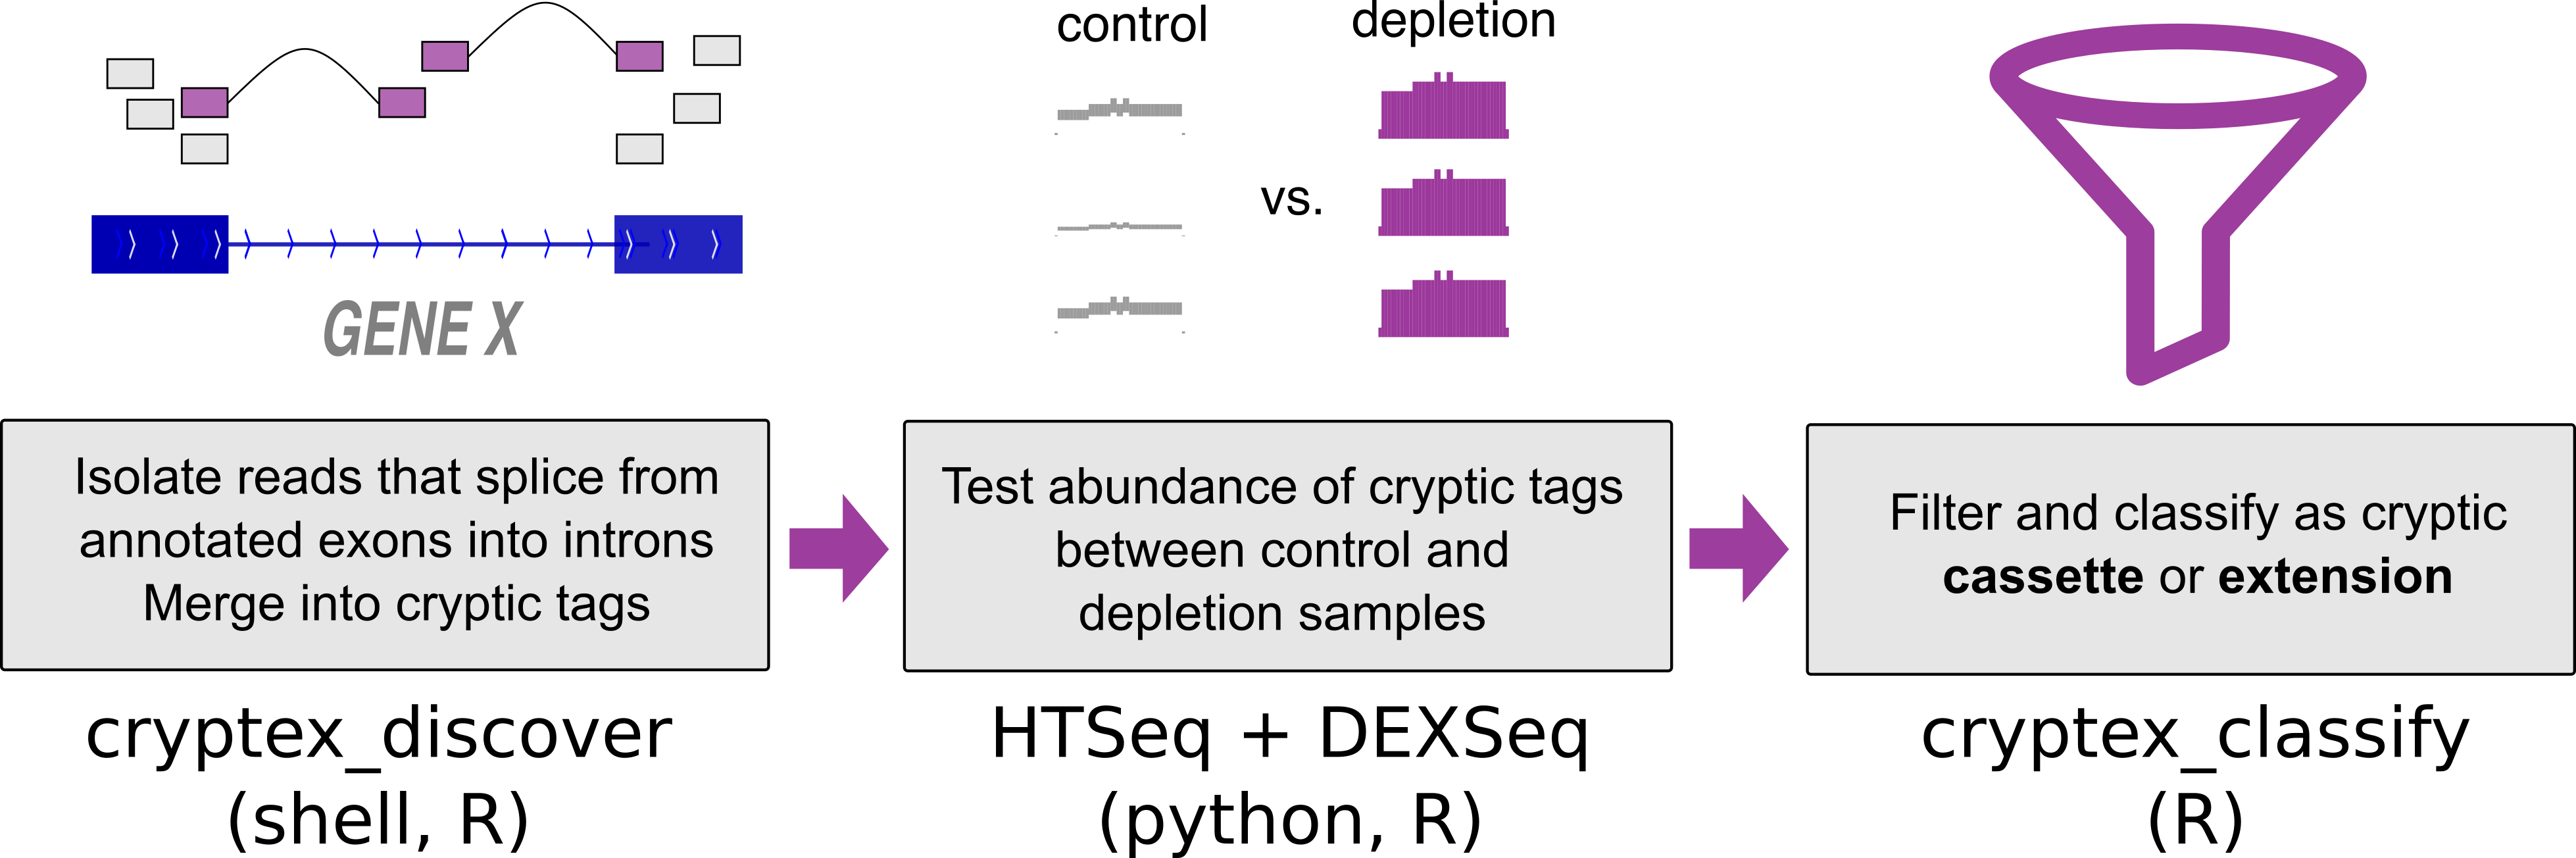
\includegraphics[width=14cm]{Figures/03_cryptic_exons/cryptex_pipeline.png}
	\caption[Schematic of the \textit{Cryptex} pipeline]{
		\textbf{Schematic of the \textit{Cryptex} pipeline}
	}
	\label{fig:cryptic_workflow}
\end{figure}

In order to discover all possible splice junctions that travel into the intron, spliced reads were extracted from each aligned bam file using \emph{SAMTools}, discarding any secondary alignments. To extract only the spliced reads that overlap an annotated exon the lists of spliced reads were intersected in \emph{BEDTools} with a flattened list of exons, created using the \url{dexseq\_prepare\_annotation.py} Python script included with the \emph{DEXSeq} package \citep{Anders2012}. An inverse intersection was then performed with the same exon list to retain only the spliced reads which do not bridge two annotated exons. The intronic mapping sections of each read were split off from the rest and retained, thus keeping a set of aligned reads that splice to, but are not part of, an annotated exon. The results of this for each sample were merged together irrespective of condition. Split reads that were within 500bp of each other were merged into larger intervals, hereby referred to as tags. This ideally captures both the upstream and downstream splice junction to a central cryptic cassette exon.  To keep only the tags that are splicing within the gene body another intersection was performed with a list of introns. This was generated from the same flattened exon file by an R script written by Devon Ryan (\url{seqanswers.com/forums/showthread.php?t=42420}). The tags were then incorporated into the flattened list of exons, the GFF file. Each tag was given a unique identification number including a reference to the upstream annotated exon, allowing for comparisons of different datasets. The reads that overlap annotated exons and tags were counted using \textit{HTSeq} \citep{Anders2015-wz} on the default settings, ignoring reads marked as PCR duplicates. The read counts were used to calculate differential usage of each exon with respect to condition with \textit{DEXSeq}. 

All the cryptic tags with an adjusted P-value (false discovery rate) $<$ 5\% and a $|\log_{2}$(fold change)$| > 0.6$ were extracted from the \textit{DEXSeq} results table. The splice junctions from the alignment of each sample were used to work out the coordinates of the canonical junction that spans the intron within which the cryptic tag is or isn't spliced in control samples. Using splice junctions from the depletion condition samples, the upstream and downstream junctions that connect the adjacent annotated exons to the cryptic tag were re-discovered and quantified. Any cryptic example that did not have at least one upstream or downstream junction per sample or had fewer than ten canonical splice junctions was removed. These junctions were used to calculate per-condition mean Percent Spliced In (PSI) values which are a ratio of cryptic splicing over the sum of cryptic and canonical splicing \citep{Katz2010-ir}. As a number of cryptic splicing events are present at a low level in control samples, $\Delta$PSI values were created for both upstream and downstream splicing for each tag. This is the difference in PSI between the depletion samples and the control samples. Any cryptic tag that had either an upstream or downstream $\Delta$PSI $<$ 5\% was removed.


\subsection{iCLIP/eCLIP enrichment}

I downloaded lists of iCLIP and eCLIP peaks (see Table \ref{table:cryptic_data}) and used the UCSC LiftOver tool to convert the coordinates into the human build 38 and mouse build 10.
The coordinates of each cryptic tag were flanked by 100 base pairs on either side to capture binding around the putative splice sites. In order to compare the overlap between cryptic exons and RNA-protein binding peaks, two sets of null exons were created for comparison, which maintain the same length as their corresponding cryptic exon but sample either the intronic sequence outside of the flanked exon or that of the adjacent introns within the same gene if available. Overlaps between exons and iCLIP and eCLIP peaks were calculated using BedTools. The proportions of overlap between the cryptic exons and the two sets of null exons were compared using a proportion test with the null hypothesis that the proportion of exons overlapping an iCLIP or eCLIP peak would be the same.

\subsection{Motif enrichment analysis}
FASTA sequence was generated for the cryptic exons flanked by 100 nucleotides either side and submitted to the \emph{MEME} web tool \citep{Bailey2009-lw} under the default settings. The analysis was repeated using the \emph{HOMER} algorithm \citep{Heinz2010-ym} on RNA mode. Motifs were created using \emph{WebLogo} \citep{Crooks2004-yg}. Frequencies of the 16 possible dinucleotides were compared between flanked cryptic exon sequences with adjacent intron sequences from the same set of genes.

\subsection{Transposable element enrichment} 
Lists of transposable elements in human and mouse (hg38 and mm10 respectively) were previously generated by the \emph{RepeatMasker} tool \citep{Smit_AFA_Hubley_R_Green_P2015-ye} and were downloaded from UCSC. Overlap between different transposable elements and the cryptic exons was calculated in each orientation using \emph{BedTools}. 

\subsection{Conservation analysis}
\textit{PhyloP} compares the sequence alignments of multiple species to produce per base conservation scores \citep{Pollard2010-fj}. Average conservation score per cryptic tag was calculated using \emph{bigWigSummary} (UCSC) for both human and mouse data. The lists of splice junctions created by \emph{STAR} when aligning each sample were used to identify the coordinates of the exons adjacent to the cryptic exon. The randomly sampled intronic sequence from the cryptic-containing intron was used as a negative control.

\subsection{Protein prediction analysis}
Any cryptic exon which did not fall within the coding sequence of a transcript was omitted. Splice junctions were used to determine the upstream and downstream exons adjacent to each cryptic exon. These exons were matched to their corresponding annotated exon in the Ensembl transcript file for each species to work out the correct frame of translation. Nucleotide sequences for transcripts either including or excluding the cryptic tag were created. If the cryptic exon had been previously flagged as an extension then the entire continuous intronic sequence was inserted up to the remaining cryptic splice site. These transcripts were then translated \textit{in silico} and defined as premature termination codon (PTC)-containing if the inclusion transcript contained a stop codon and as a frameshift if the sequence of the downstream exon no longer matched. A null distribution of PTC-containing or frame shifted transcripts was created by shuffling the identity of the central exon 1000 times. 

\subsection{Splice junction scoring }
The strength of 5\'\ and 3\'\ splice sites was calculated for the human cryptic exons using \emph{maxEnt} \citep{Yeo2004-pz}. Higher scores indicate the increased log odds of a given splice site being a true splice site. The 5\'\ splice site is defined as the last 3 nucleotides of the upstream exon flanked by 6 intronic nucleotides, of which the first two are invariably GU. The 3\'\ splice site is defined as the last 20 intronic nucleotides of which the final two are invariably AG, flanked by the first 3 nucleotides of the downstream exon. The splice sites of annotated exons were used as a positive control. Randomly generated sequence with invariant AG or GT was used as a negative control. Paired t-tests were carried out to test the direction of change between the cryptic and annotated splice sites for each class of cryptic exon.


\section{Results}
\subsection{Depletion of TDP-43 but not FUS results in cryptic exons}

I downloaded and analyzed 9 publicly available RNA-seq datasets (Table \ref{table:cryptic_data}. 
This comprised TDP-43 depletion (three human and three murine, datasets 1-6), FUS depletion (1 human, 1 murine, datasets 7-8) and as a positive control a human hnRNP C depletion dataset for which cryptic exons have previously been reported (dataset 9).  
While these datasets differ in library preparation method, read depth and length, and protein depletion method (Table \ref{table:cryptic_sequence_stats}), the FUS datasets match the TDP-43 datasets by cell type. 

\begin{figure}[h!]
	\centering
	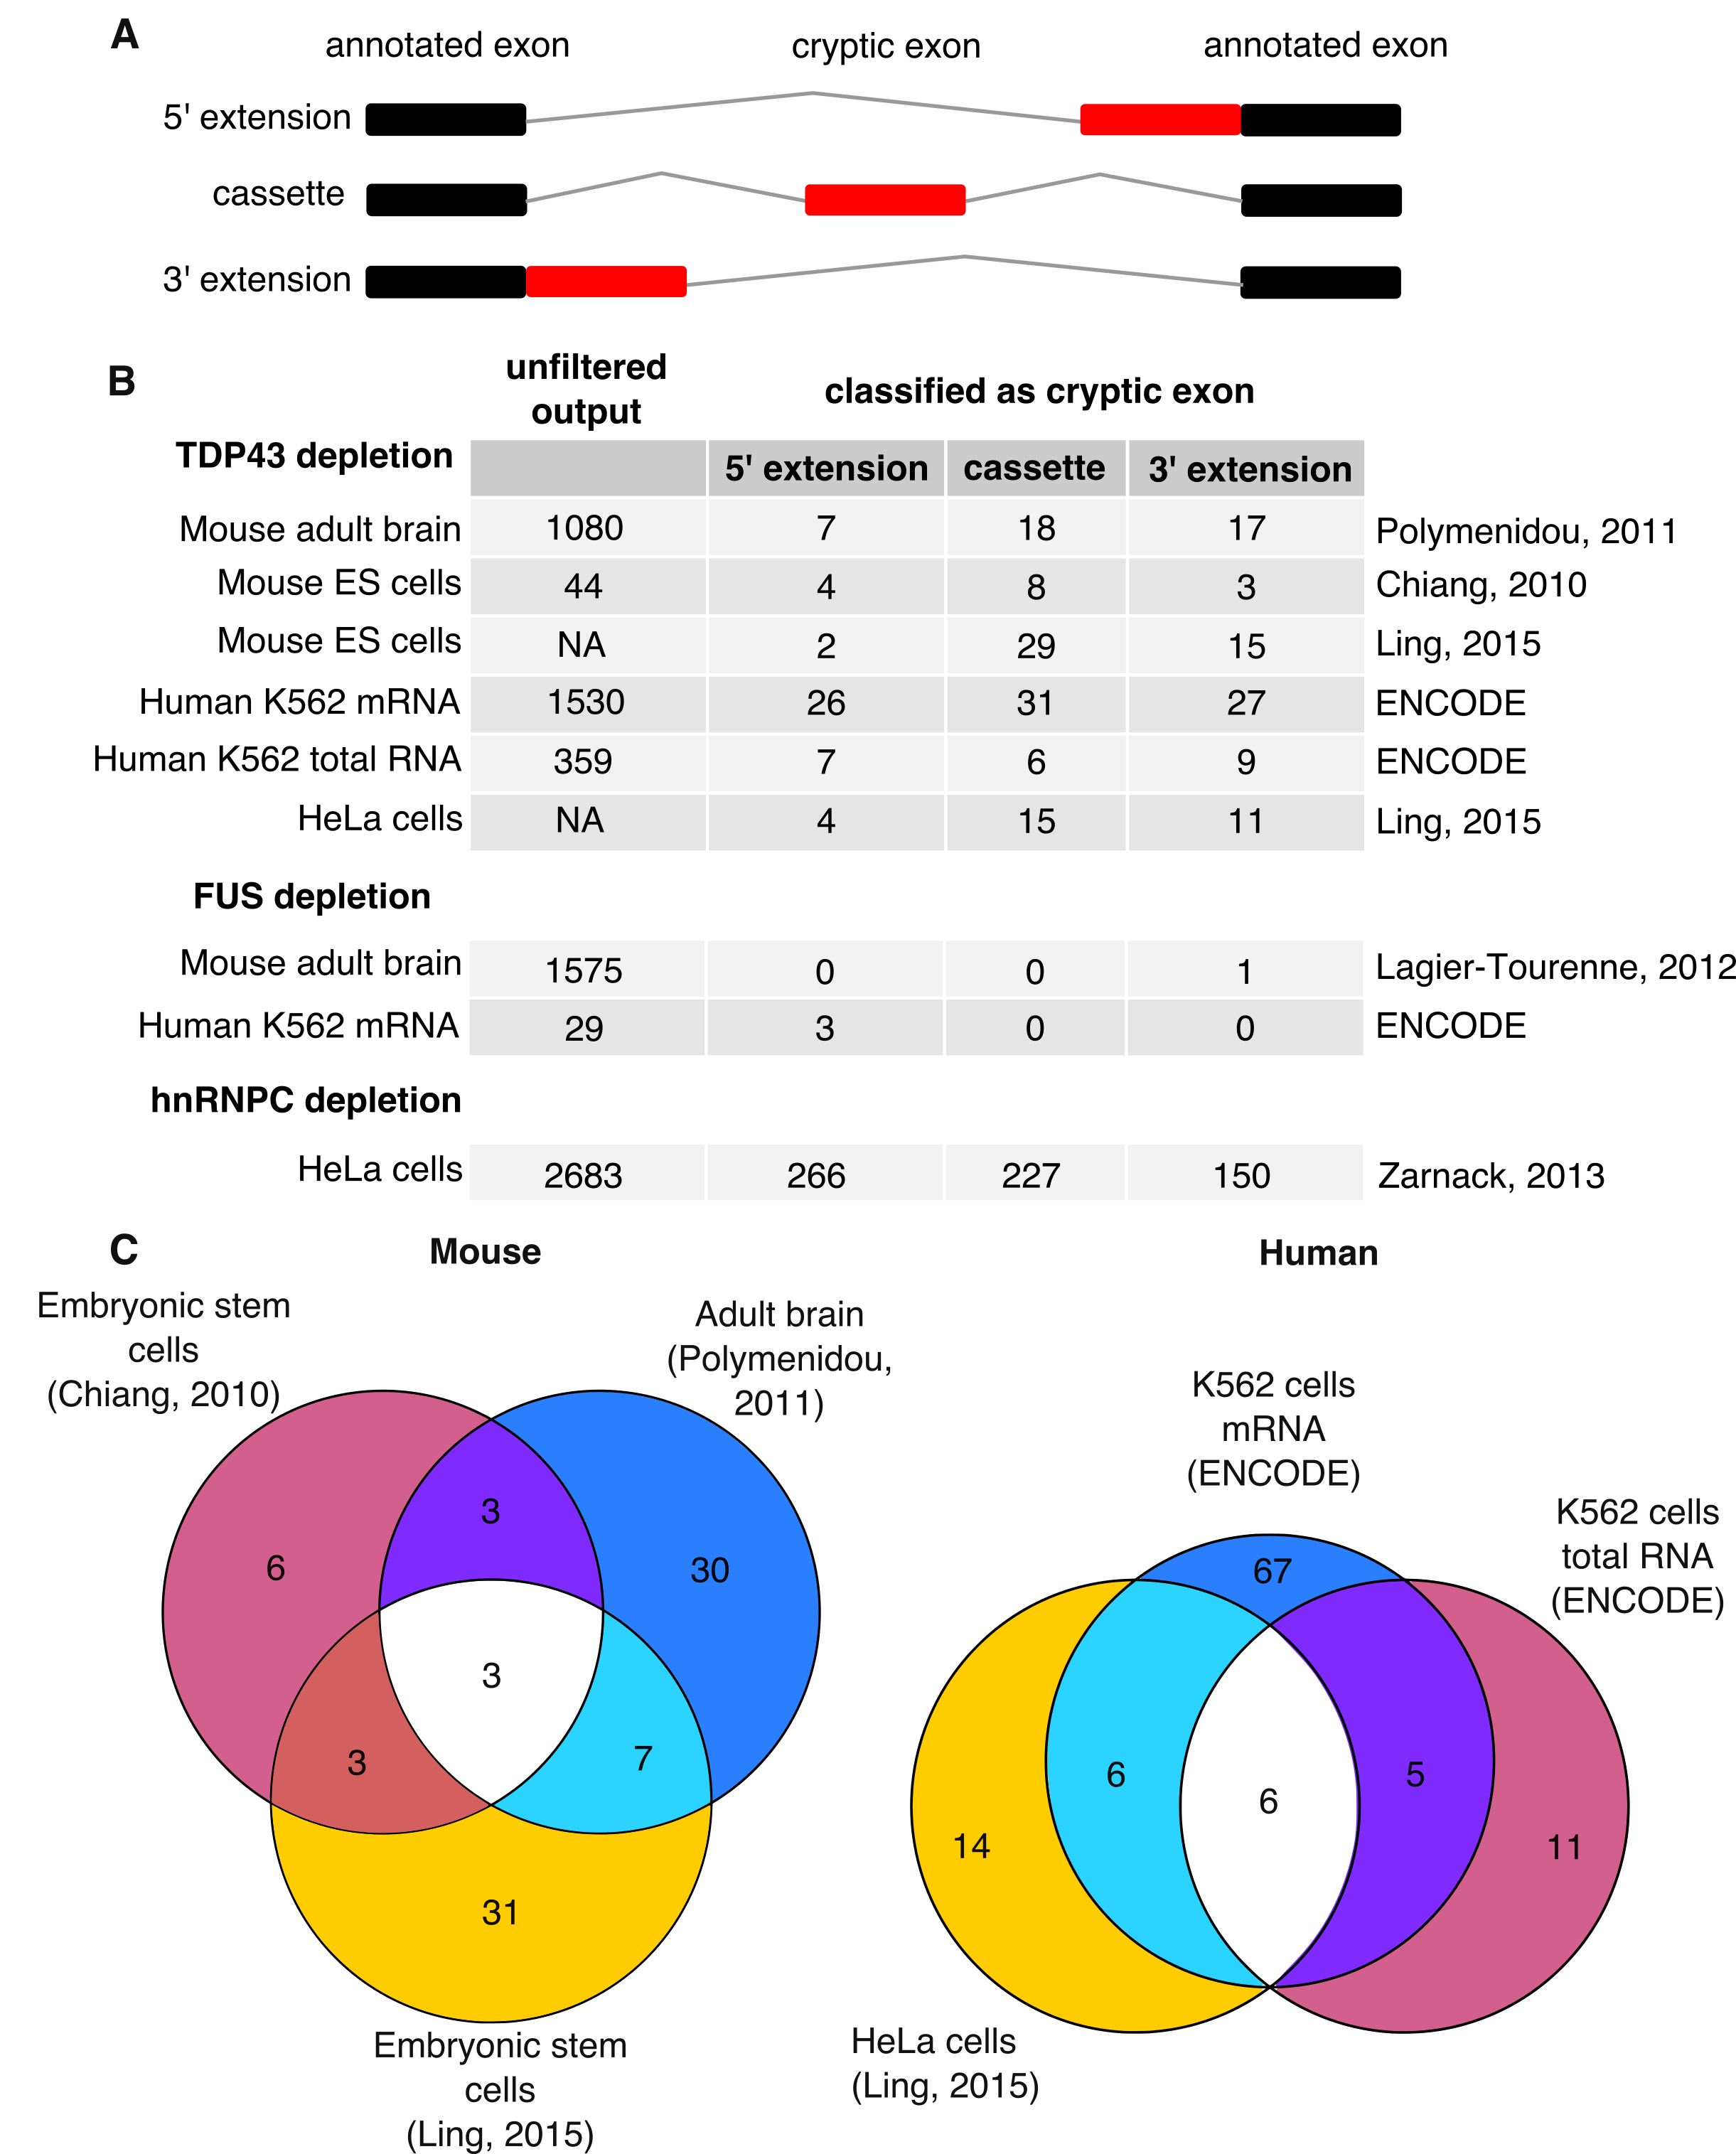
\includegraphics[width=\textwidth]{Figures/03_cryptic_exons/Figure_1_venn_inkscape.png}
	\caption[Cryptic splicing discovered by the \emph{CryptEx} pipeline]{
		\textbf{Cryptic splicing discovered by the \emph{CryptEx} pipeline}
	\textbf{(A)} Schematic of the three classes of cryptic exon. Black boxes represent annotated exons and red boxes represent a cryptic exon. Grey lines represent the spliced intron. 
	\textbf{(B)} Tally of the three classes of cryptic exon discovered by the Cryptex pipeline across the nine datasets. ``Unfiltered output'' refers to the number of differentially used cryptic splicing events at a false discovery rate (FDR) $<$ 5\% before undergoing cryptic exon classification. Counts from Ling et al's data are taken from the paper itself. 
	\textbf{(C)} Venn diagrams showing the overlap between the six TDP-43 depletion datasets.
}
	\label{fig:cryptic_venn}
\end{figure}

Significant cryptic exons discovered by \textit{Cryptex} were classified into three categories: (i) cassette-like, where novel 3\'\ and 5\'\ splice sites are recognised, which forms a completely new exon; (ii) 5\'\ extension, where a novel 3\'\ splice site is recognised and an existing exon is extended upstream of its annotated start and (iii) 3\'\ extension, where a novel 5\'\ splice site is recognised and an exon is extended downstream of its annotated end (Fig. \ref{fig:cryptic_venn}A). 
\textit{Cryptex} does not consider fully retained introns, but other methods have been designed for this purpose \citep{Li2015a,Bai2015-aq,Braunschweig2014}.

Comparing the two human ENCODE K562 cell line TDP-43 depletion datasets (3-4), the poly-A selected mRNA-Seq dataset yielded far more splicing events than the total RNA dataset, presumably due to polyA+ selection leading to a higher coverage of mature spliced mRNA species (Fig. \ref{fig:cryptic_venn}B). In total 95 human cryptic exons were discovered and classified, with the majority only detected in the mRNA-seq dataset. 11 cryptic splicing events were shared between datasets 3 and 4 (Fig. \ref{fig:cryptic_venn}C). Of the 26 human cryptic exons reported by Ling, 12 were detected in at least one of the two datasets 3 and 4. 

Both mouse datasets differ in both cell type (adult striatum in dataset 5 vs embryonic stem (ES) cell in dataset 6) and read depth (35-60M in dataset 5 vs 2-10M in dataset 6). 52  cryptic exons were identified in total, with 46 detected in the adult striatum and 15 in ES cells, with 6 exons observed in both. Of the 46 cryptic splicing events identified in murine samples by Ling et al, 13 were detected in at least one of datasets 5 and 6. Side by side visual inspection suggests that differences in library preparation and read depth are behind the low  concordance rates in both human and mouse, as cryptic exons detected in the higher depth dataset (K562 mRNA and mouse adult brain) can be observed by eye in the lower depth dataset (K562 total RNA and mouse ES cell). These exons currently fail to be detected by the \emph{CryptEx} algorithm.

No cryptic splicing events were shared between human and mouse as previously reported \citep{Ling2015}. Note that to report overlap with Ling and colleagues (datasets 1 and 2), the raw data was unsuitable for the cryptic exon discovery pipeline due to a lack of biological replicate samples. Instead the sequence data was aligned and the splice junctions generated by the aligner were used to classify previously reported cryptic exons.

In contrast, while a large number of novel splicing events were observed in the FUS depletion datasets, our algorithm only classified 3 in mouse and 1 in human as cryptic exons. FUS depletion was not observed to produce any cassette-like cryptic exons in either species. The coordinates of each cryptic exon found in human and mouse are reproduced in the appendices.

\subsection{Cryptic exons are bound by TDP-43}

\begin{figure}[h!]
	\centering
	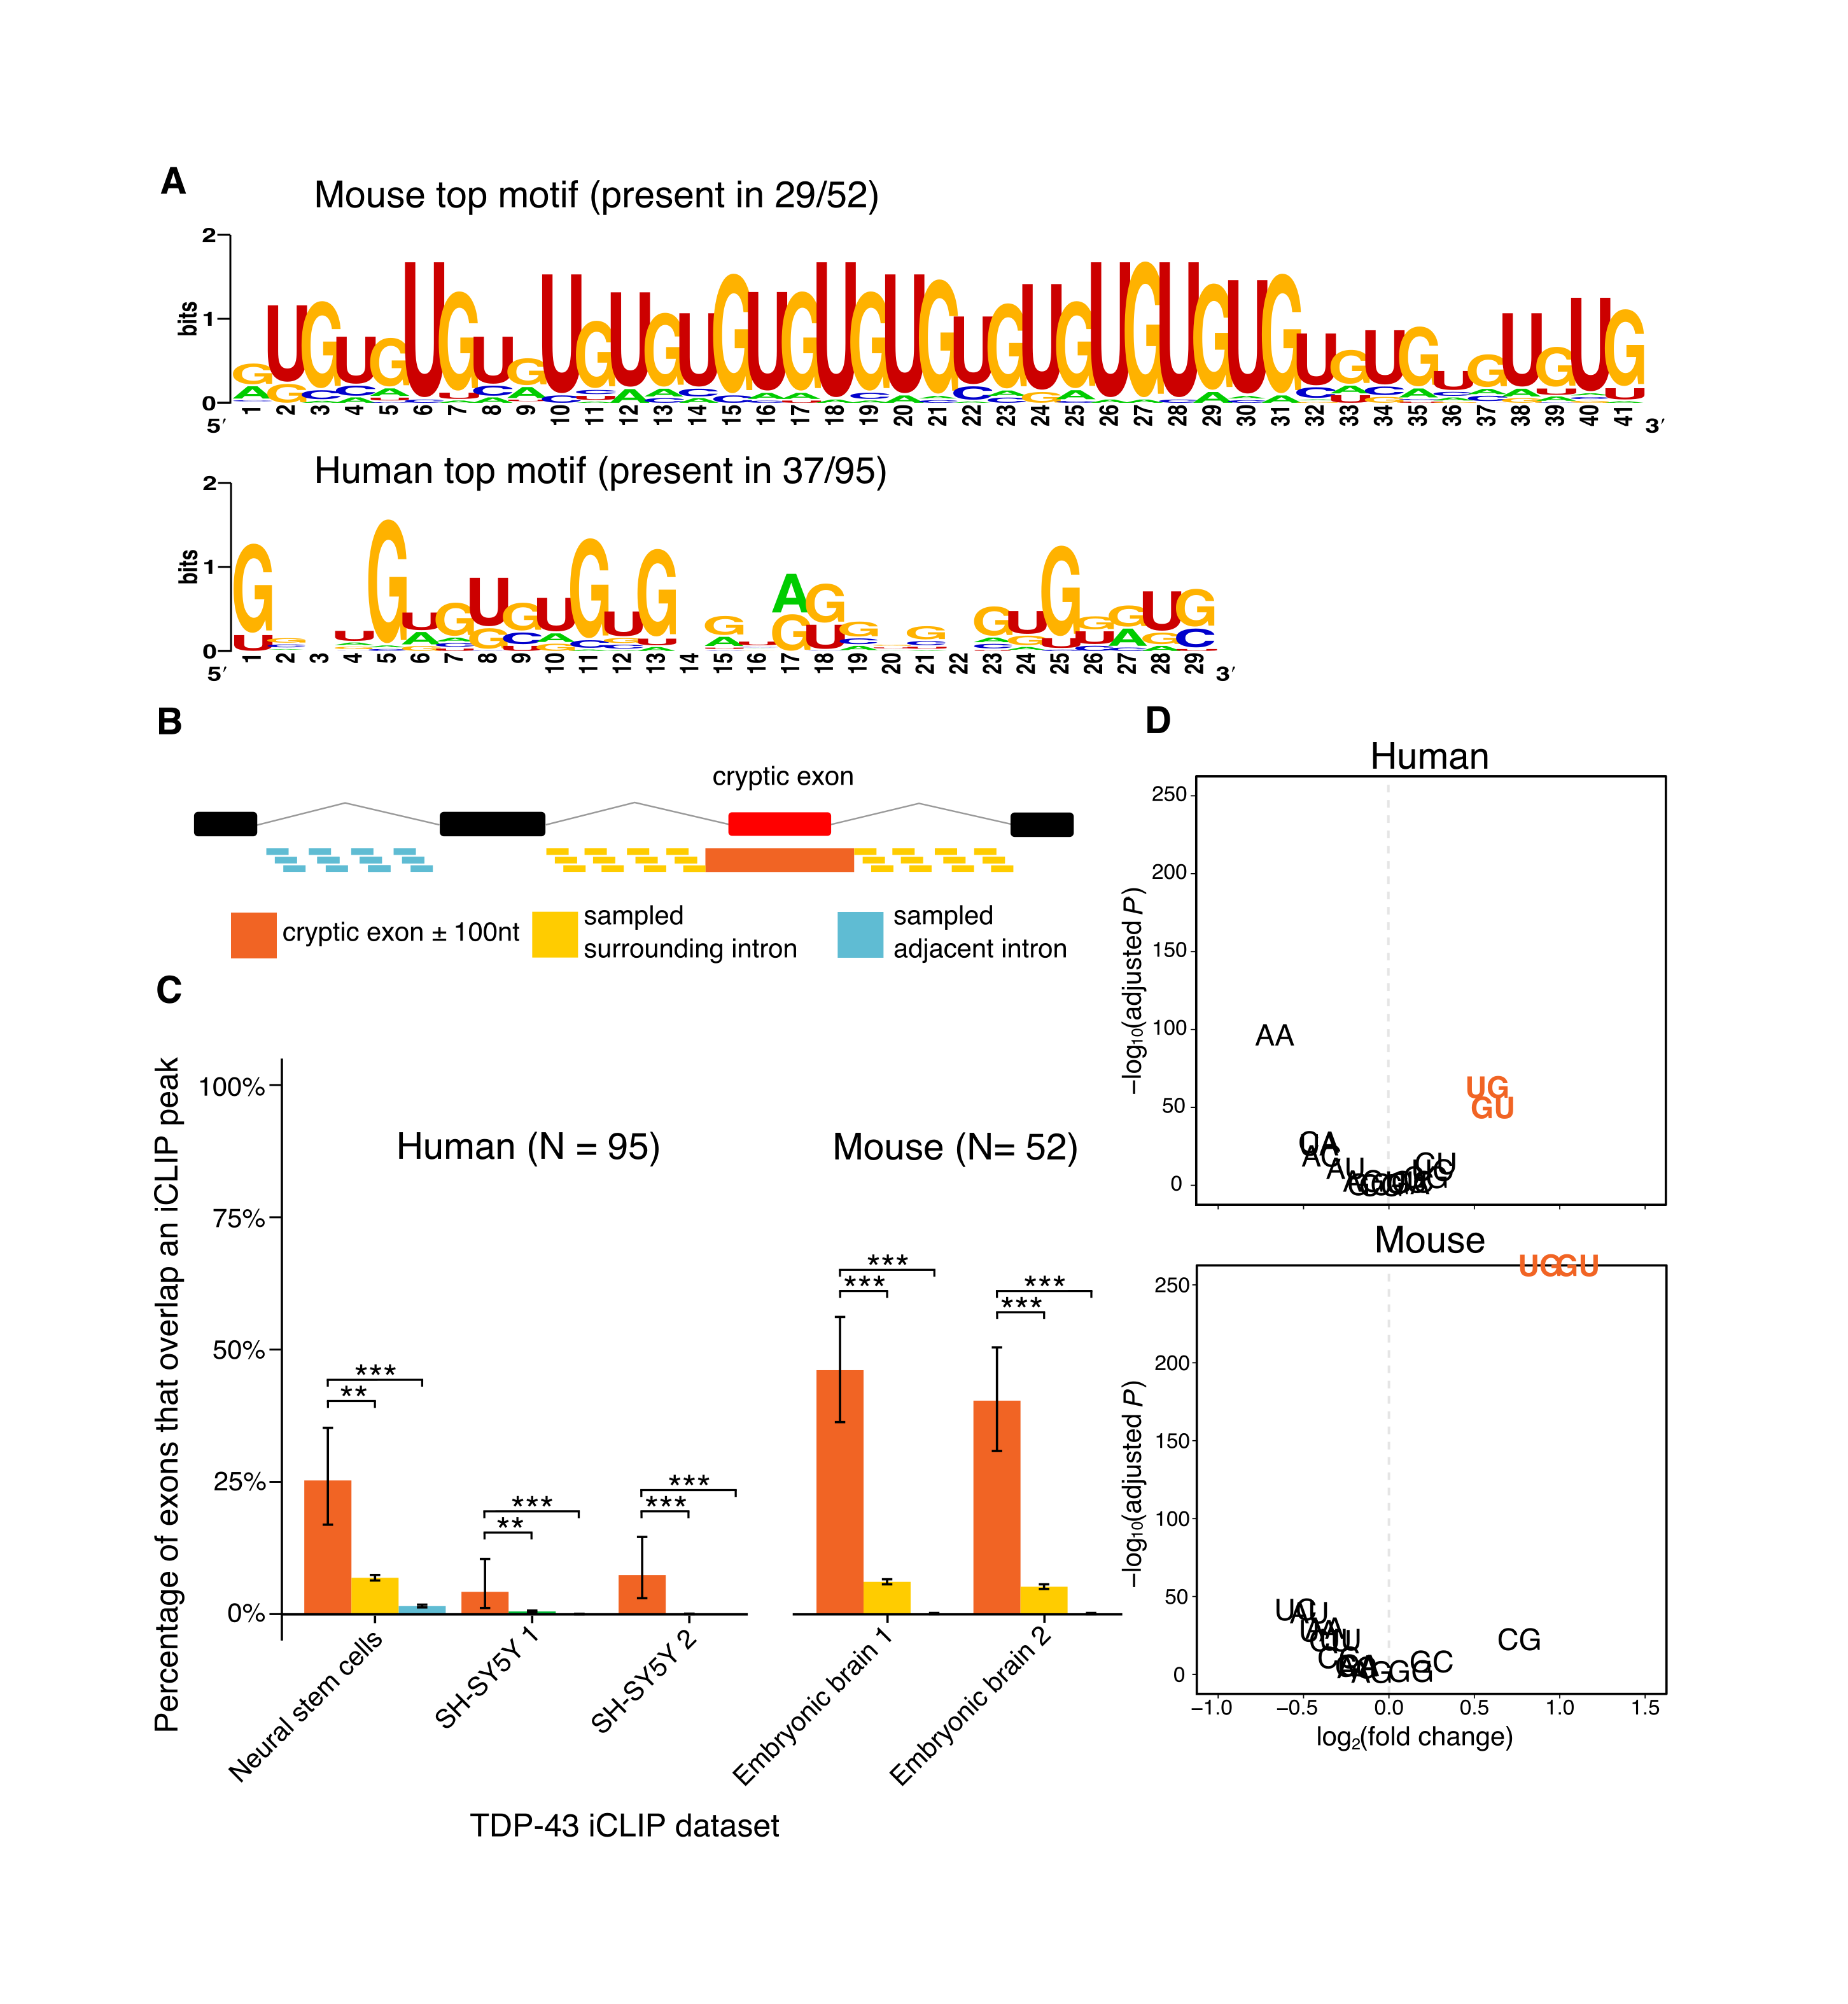
\includegraphics[width=\textwidth]{Figures/03_cryptic_exons/Figure_2_motif_iCLIP.png} 
	\caption[Evidence of TDP-43 binding cryptic exons]{
		\textbf{Evidence of TDP-43 binding cryptic exons.}
	\textbf{(A)} Results of \emph{MEME} motif search. Only the motif with the greatest enrichment compared to background sequence is presented. 
	\textbf{(B)} Schematic of iCLIP peak enrichment test. For illustration a cassette-like cryptic exon (green box) is shown between two annotated exons (black boxes) separated by intronic sequence (black lines). The proportion of the group of cryptic exons flanked either side by 100 nucleotides (orange) that overlap at least one iCLIP peak is compared to the proportion of overlaps in a group of length matched sequences from either the surrounding intron (yellow) or an adjacent intron (blue) each randomly sampled 100 times per gene. 
	\textbf{(C)} iCLIP peak overlap enrichment for the 95 human cryptic exons found in either K562 cell TDP-43 depletion dataset and the 52 cryptic exons found in either mouse TDP-43 depletion dataset. D) Dinucleotide enrichment in the flanked cryptic exons compared to adjacent introns. Error bars denote 95\% confidence intervals of the binomial distribution. $^* P < 0.05 $, $^{**} P < 0.001$, $^{***} P < 10^{-16}$ . All \textit{P}-values adjusted for multiple testing by Bonferroni method.
}
	\label{fig:cryptic_motifs}
\end{figure}


TDP-43 linked cryptic exons were grouped into unions of all cassette-like exons and extension events discovered in human and mouse, totalling 95 human and 52 murine cryptic exons. I then explored whether TDP-43 binding could explain the observed splicing changes in RNA-Seq data, as observed by Ling and colleagues. I took two complementary approaches: (i) searching for enriched motifs in the RNA sequence including and surrounding the cryptic exons (Fig. \ref{fig:cryptic_motifs}A,D) and (ii) correlating the positions of cryptic exons with TDP-43 protein-RNA interaction data (Fig. \ref{fig:cryptic_motifs}B,C).

TDP-43 can repress or enhance the inclusion of a given exon by either binding within or adjacent to the exonic sequence \citep{Tollervey2011}. Hence, for our motif search, I flanked cryptic exon sequences by 100 nucleotides on either side. UG-rich motifs were found to be enriched in both mouse and human cryptic exons using two different algorithms: \emph{MEME} (Fig. \ref{fig:cryptic_motifs}A) and \emph{HOMER} (appendices). Of the 52 mouse cryptic exons, 29 had a run of UG up to 40 nucleotides in length. Similarly, human cryptic exons were enriched in a UG motif but not in a continuous manner. By comparing  the frequencies of  16 possible dinucleotides between the flanked cryptic exon sequence and the sequence of the adjacent intron either up or downstream of the cryptic-containing intron it was possible to resolve the enrichment of UG dinucleotides (Fig. \ref{fig:cryptic_motifs}D). UG and GU were enriched in flanked cryptic exon sequence in both human (fold change GU = 1.53; UG = 1.48; $P < 10^{-50}$; proportion test) and mouse (fold change GU = 2.14; UG = 1.85; $P < 10^{-50}$; proportion test). 
If TDP-43 binding was uniform throughout an intron or gene then one would expect to see similar proportions of overlap between cryptic exons, surround intronic sequence and adjacent exons (Fig. \ref{fig:cryptic_motifs}B). However, both species show an enrichment in TDP-43 binding peaks specific to the cryptic exons in every iCLIP dataset used, with as much as 25\% of human cryptic exons and 50\% of mouse cryptic exons overlapping at least one iCLIP peak each (both species: $P < 10^{-16}$, proportion test) (Fig. \ref{fig:cryptic_motifs}C). 



\subsection{Cryptic exon recognition is unrelated to the binding of transposable elements by TDP-43}

\begin{figure}[h!]
	\centering
	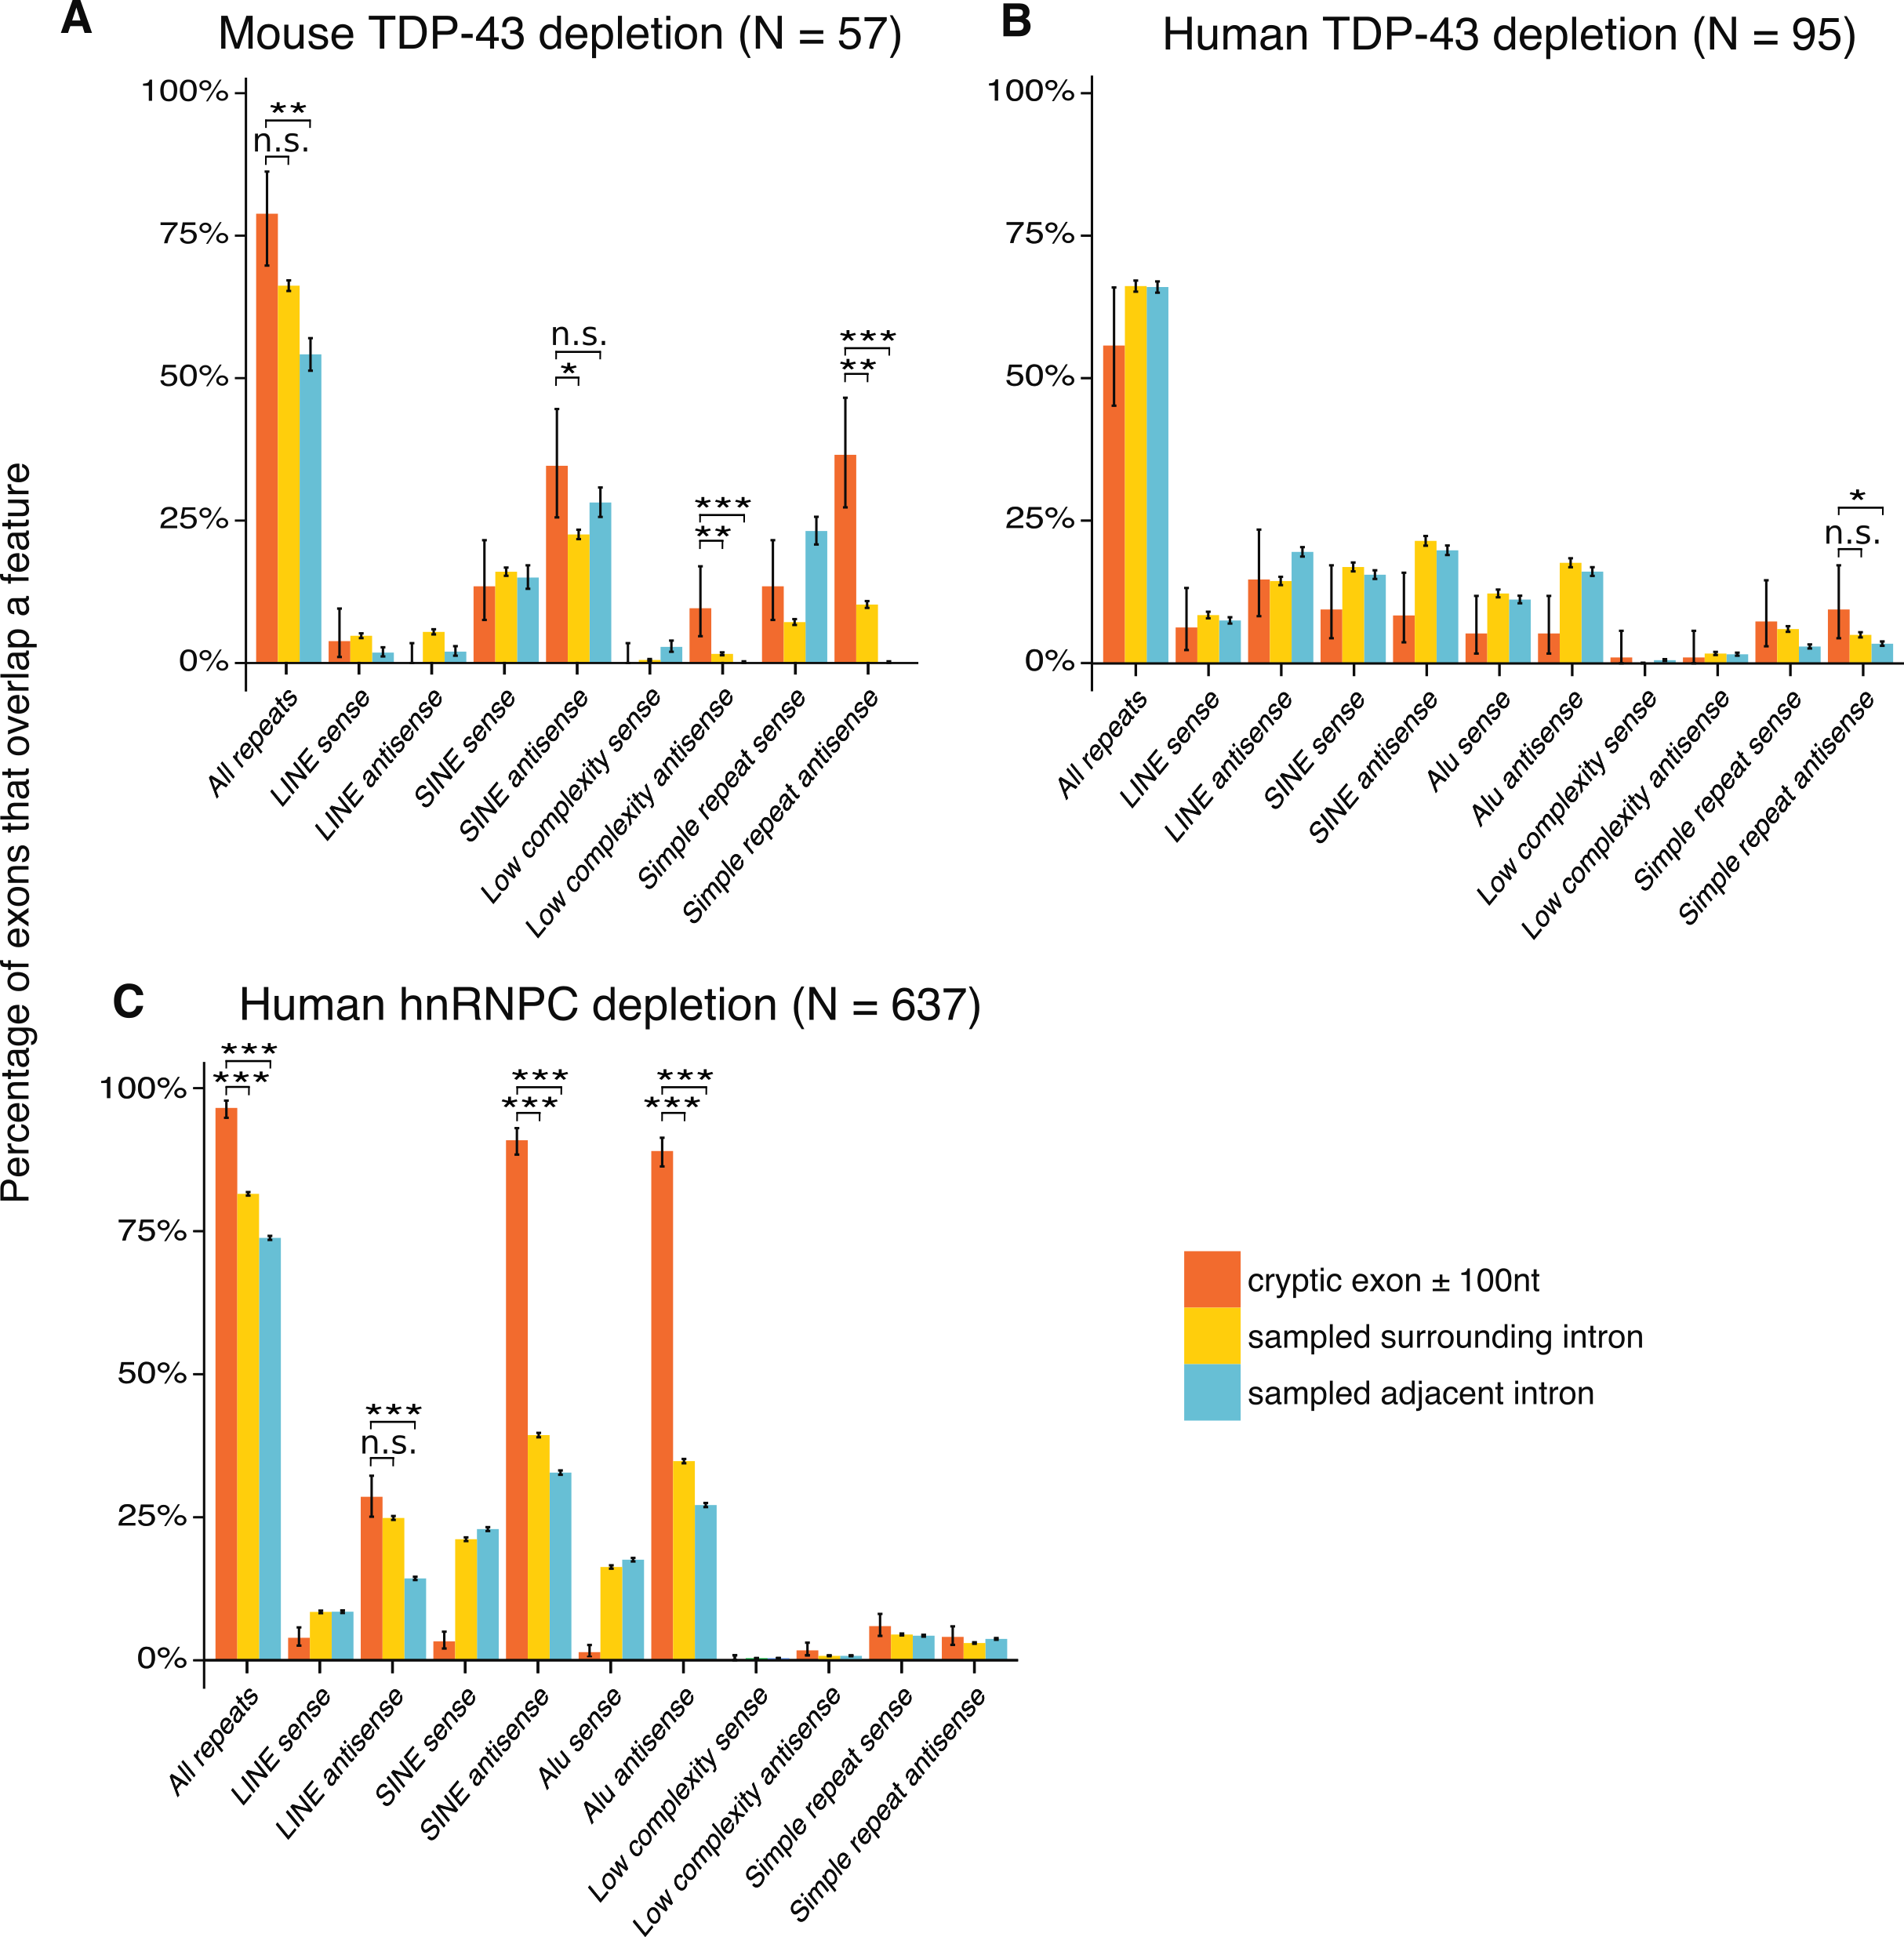
\includegraphics[width=\textwidth]{Figures/03_cryptic_exons/Figure_3_repeat_elements.png}
	\caption[Cryptic exons in transposable elements]{
		\textbf{Cryptic exons in transposable elements.}
		Overlap between different families of repetitive element with lists of exons, separated by orientation. 
		\textbf{(A)} Mouse TDP-43 depletion. 
		\textbf{(B)} Human TDP-43 depletion. 
		\textbf{(C)} Human hnRNP C depletion. 
		The proportion of the cryptic exons that contain a particular element are shown in orange. Length matched random samples from the surrounding intron (yellow) and adjacent introns (blue) are used as controls. LINE: Long Interspersed Nuclear Element; SINE: Short Interspersed Nuclear Element.  $^*: P < 0.05$, $^{**}: P < 0.001$, $^{***}: P < 10^{-16}$ . All \textit{P}-values corrected for multiple testing with Bonferroni method.
	}
	\label{fig:cryptic_repeats}
\end{figure}

TDP-43 has been demonstrated to bind antisense Alu elements, which are the source of cryptic exons repressed by hnRNP C \citep{Zarnack2013,Kelley2014-sr}. I therefore investigated whether TDP-43 induced cryptic exons preferentially overlap specific families of transposable elements and/or class of repetitive sequences. Transposable and repeat elements annotations were obtained using the \emph{RepeatMasker} software, and these features were split by family and orientation. Although Alu elements are a subfamily within the primate SINE element family, I included them separately given the prior hnRNP C result.
Control regions were obtained as before. Cryptic exons show only a modest enrichment patterns in the simple repeat" family, owing to the aforementioned UG motifs (Fig. \ref{fig:cryptic_repeats}A/B). This contrasts with hnRNP C depletion, which shows a striking enrichment of antisense SINE elements of which all are of the Alu type ($P < 10^{-16}$, proportion test; Fig. \ref{fig:cryptic_repeats}C), a result consistent with previous analyses of dataset 9 \citep{Zarnack2013}.

\subsection{Cryptic exons are poorly conserved and generate premature stop codons}

\begin{figure}[h]
	\centering
	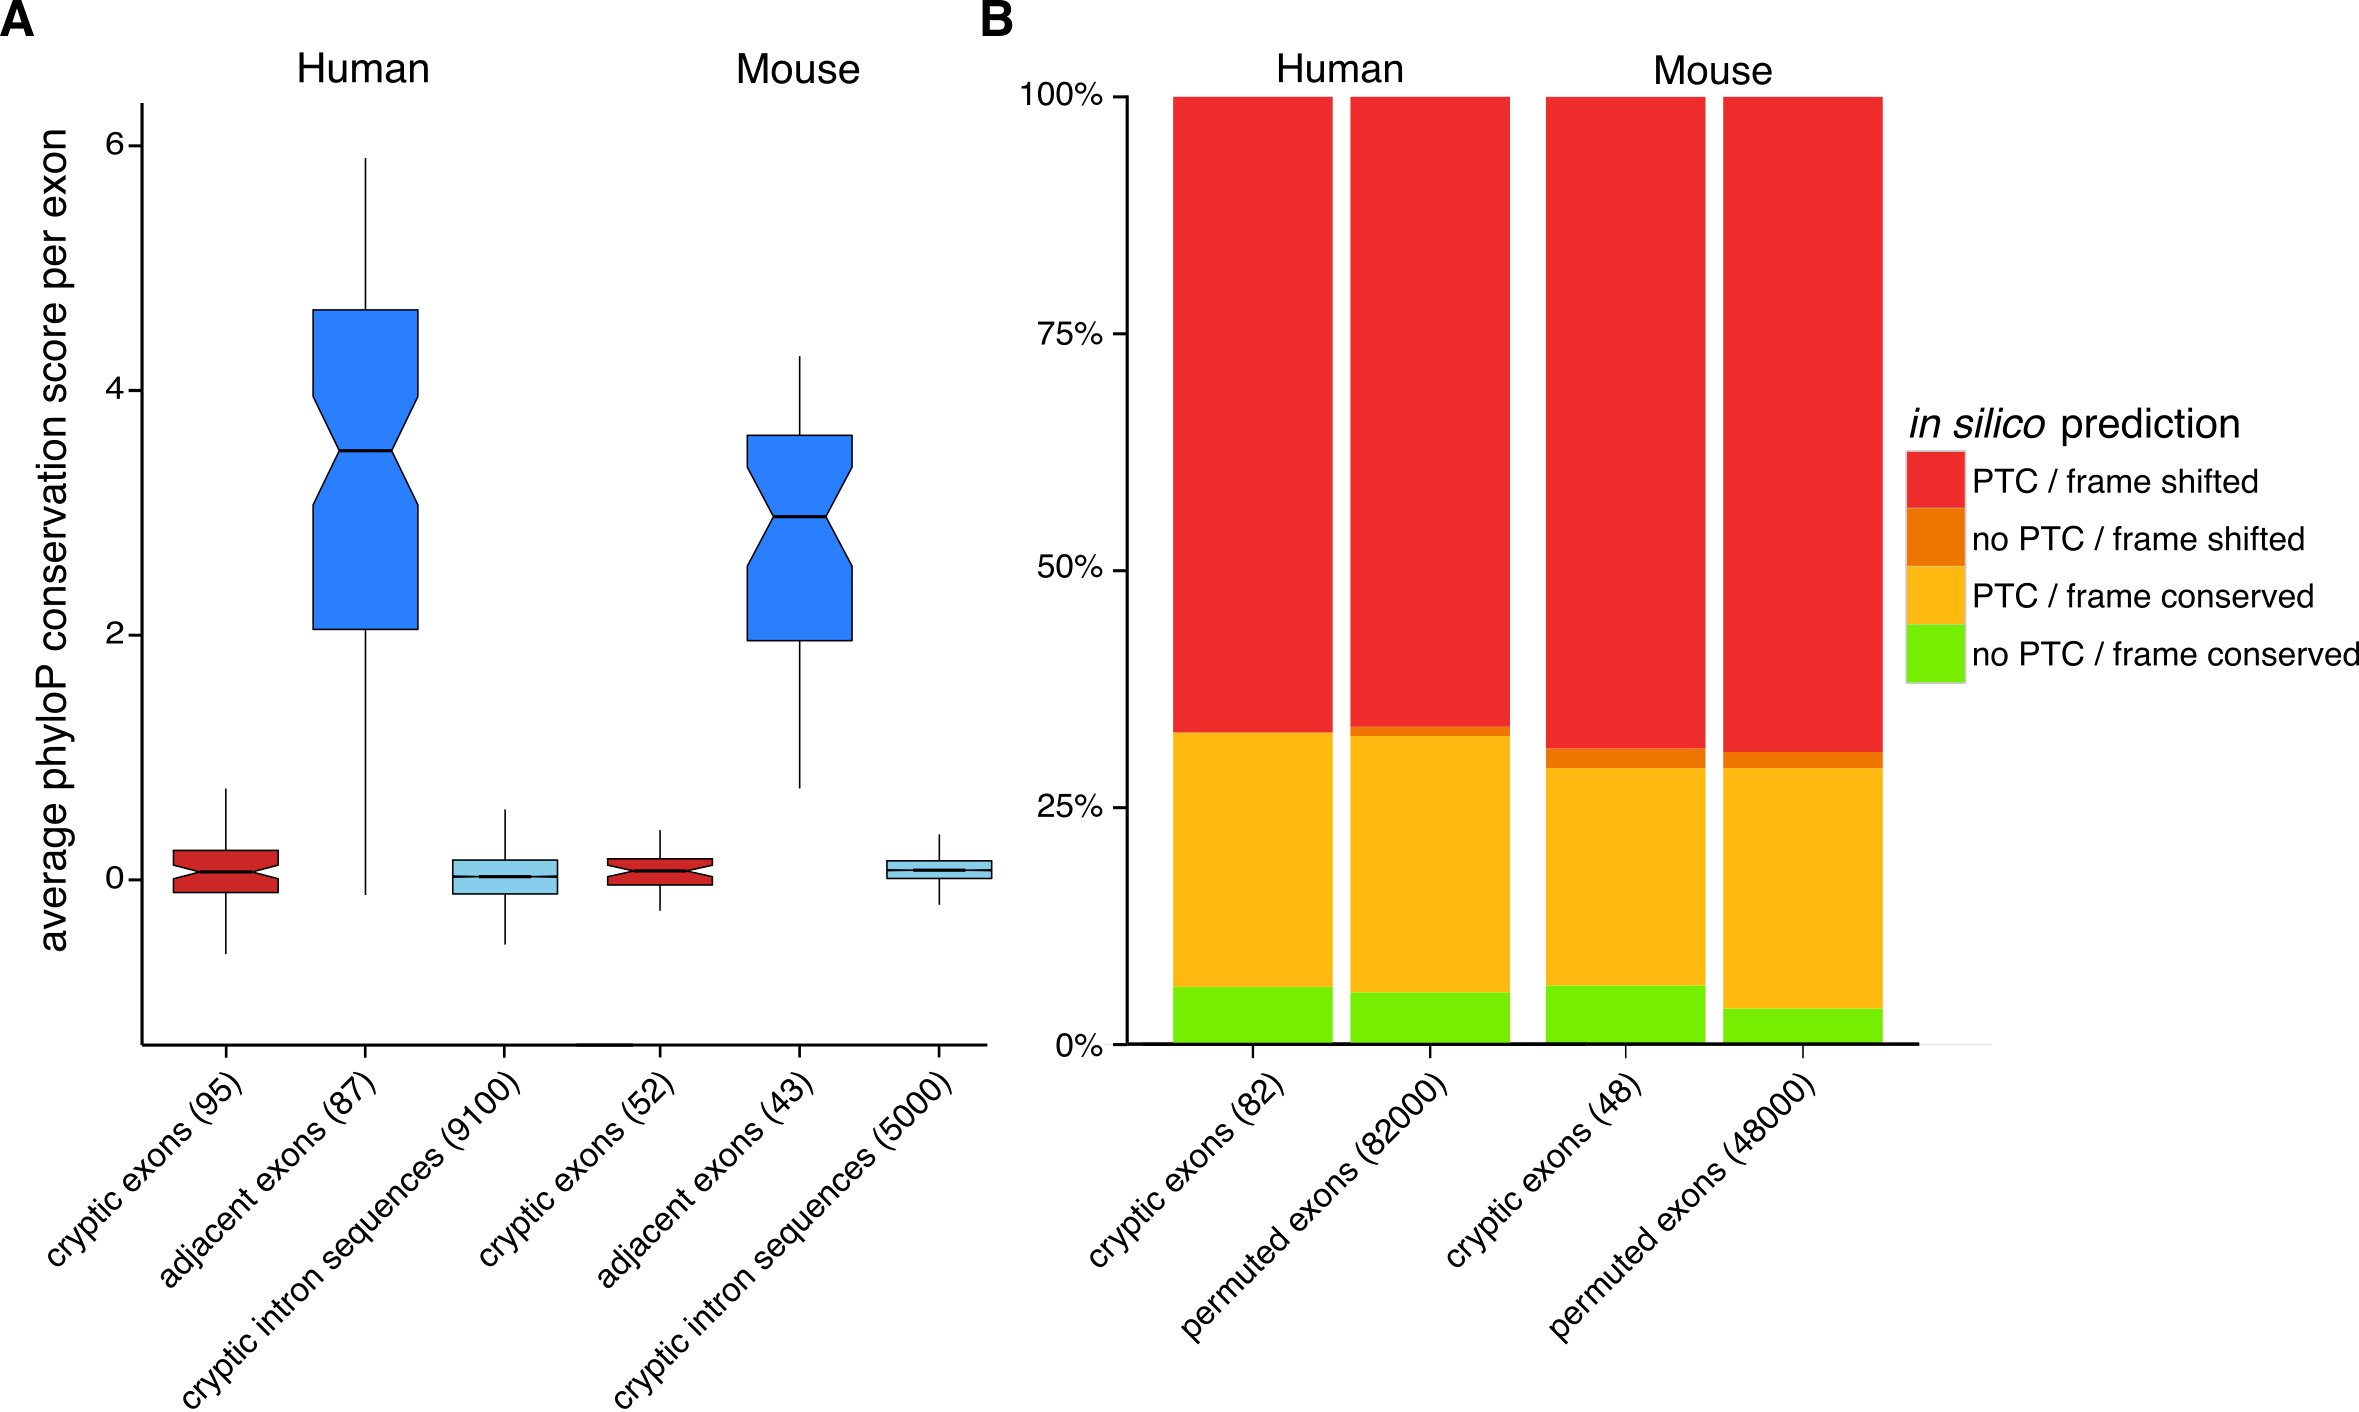
\includegraphics[width=\textwidth]{Figures/03_cryptic_exons/Figure_4_conservation_poison.png}
	\caption[Conservation and premature termination codon analysis]{
		\textbf{Conservation and premature termination codon analysis.}
		\textbf{(A)} Per exon average PhyloP conservation scores in cryptic exons, adjacent exons within the same set of genes (when available) and randomly sampled sequences from the cryptic containing intron. Box plots show first quartile, median and third quartile with the notches representing the 95\% confidence interval of the median. Whiskers represent the minimum and maximum values that fall within 1.5 times the interquartile range. 
		\textbf{(B)} The functional impact of cryptic exon inclusion on the host transcripts in human and mouse. Colours indicate the category of prediction and box size indicates the proportion of the total group of exons in each category. Categories from top to bottom: at least one premature termination codon (PTC) introduced and frame shifted (red); no PTCs introduced but frame shifted (orange); PTCs introduced but frame conserved (yellow); no PTCs introduced and frame conserved (green). For each species there is a corresponding set of null exons where the central exon has been permuted 1000 times.
}
	\label{fig:cryptic_conservation}
\end{figure}

I then quantified the extent of evolutionary conservation of cryptic exons using the multiple species alignment conservation scores generated by \textit{PhyloP}. I calculated mean conservation scores per exon for the cryptic exons and compared them to scores from both the annotated exons and randomly sampled intronic sequences from the same genes. No differences were observed between cryptic exons and matched intronic sequences (Fig. \ref{fig:cryptic_conservation}A), and a much lower conservation level than adjacent annotated exons.

I also investigated the consequences of inclusion of cryptic exons on translation of the transcript. Potential outcomes for each gene are: (i) a functional transcript, (ii) a premature termination code (PTC) or (iii) a frameshift variant. I compared these estimates to random simulations where the identity of the included exon has been permuted 1000 times. The results were consistent with the null expectation, with around 66\% of cryptic exons leading to a frameshift due to length mismatches and less than 10\% of cryptic exons predicted to create functional transcripts (Fig. \ref{fig:cryptic_conservation}B).


\subsection{Cryptic exon containing genes are downregulated}

\begin{figure}[h!]
	\centering
	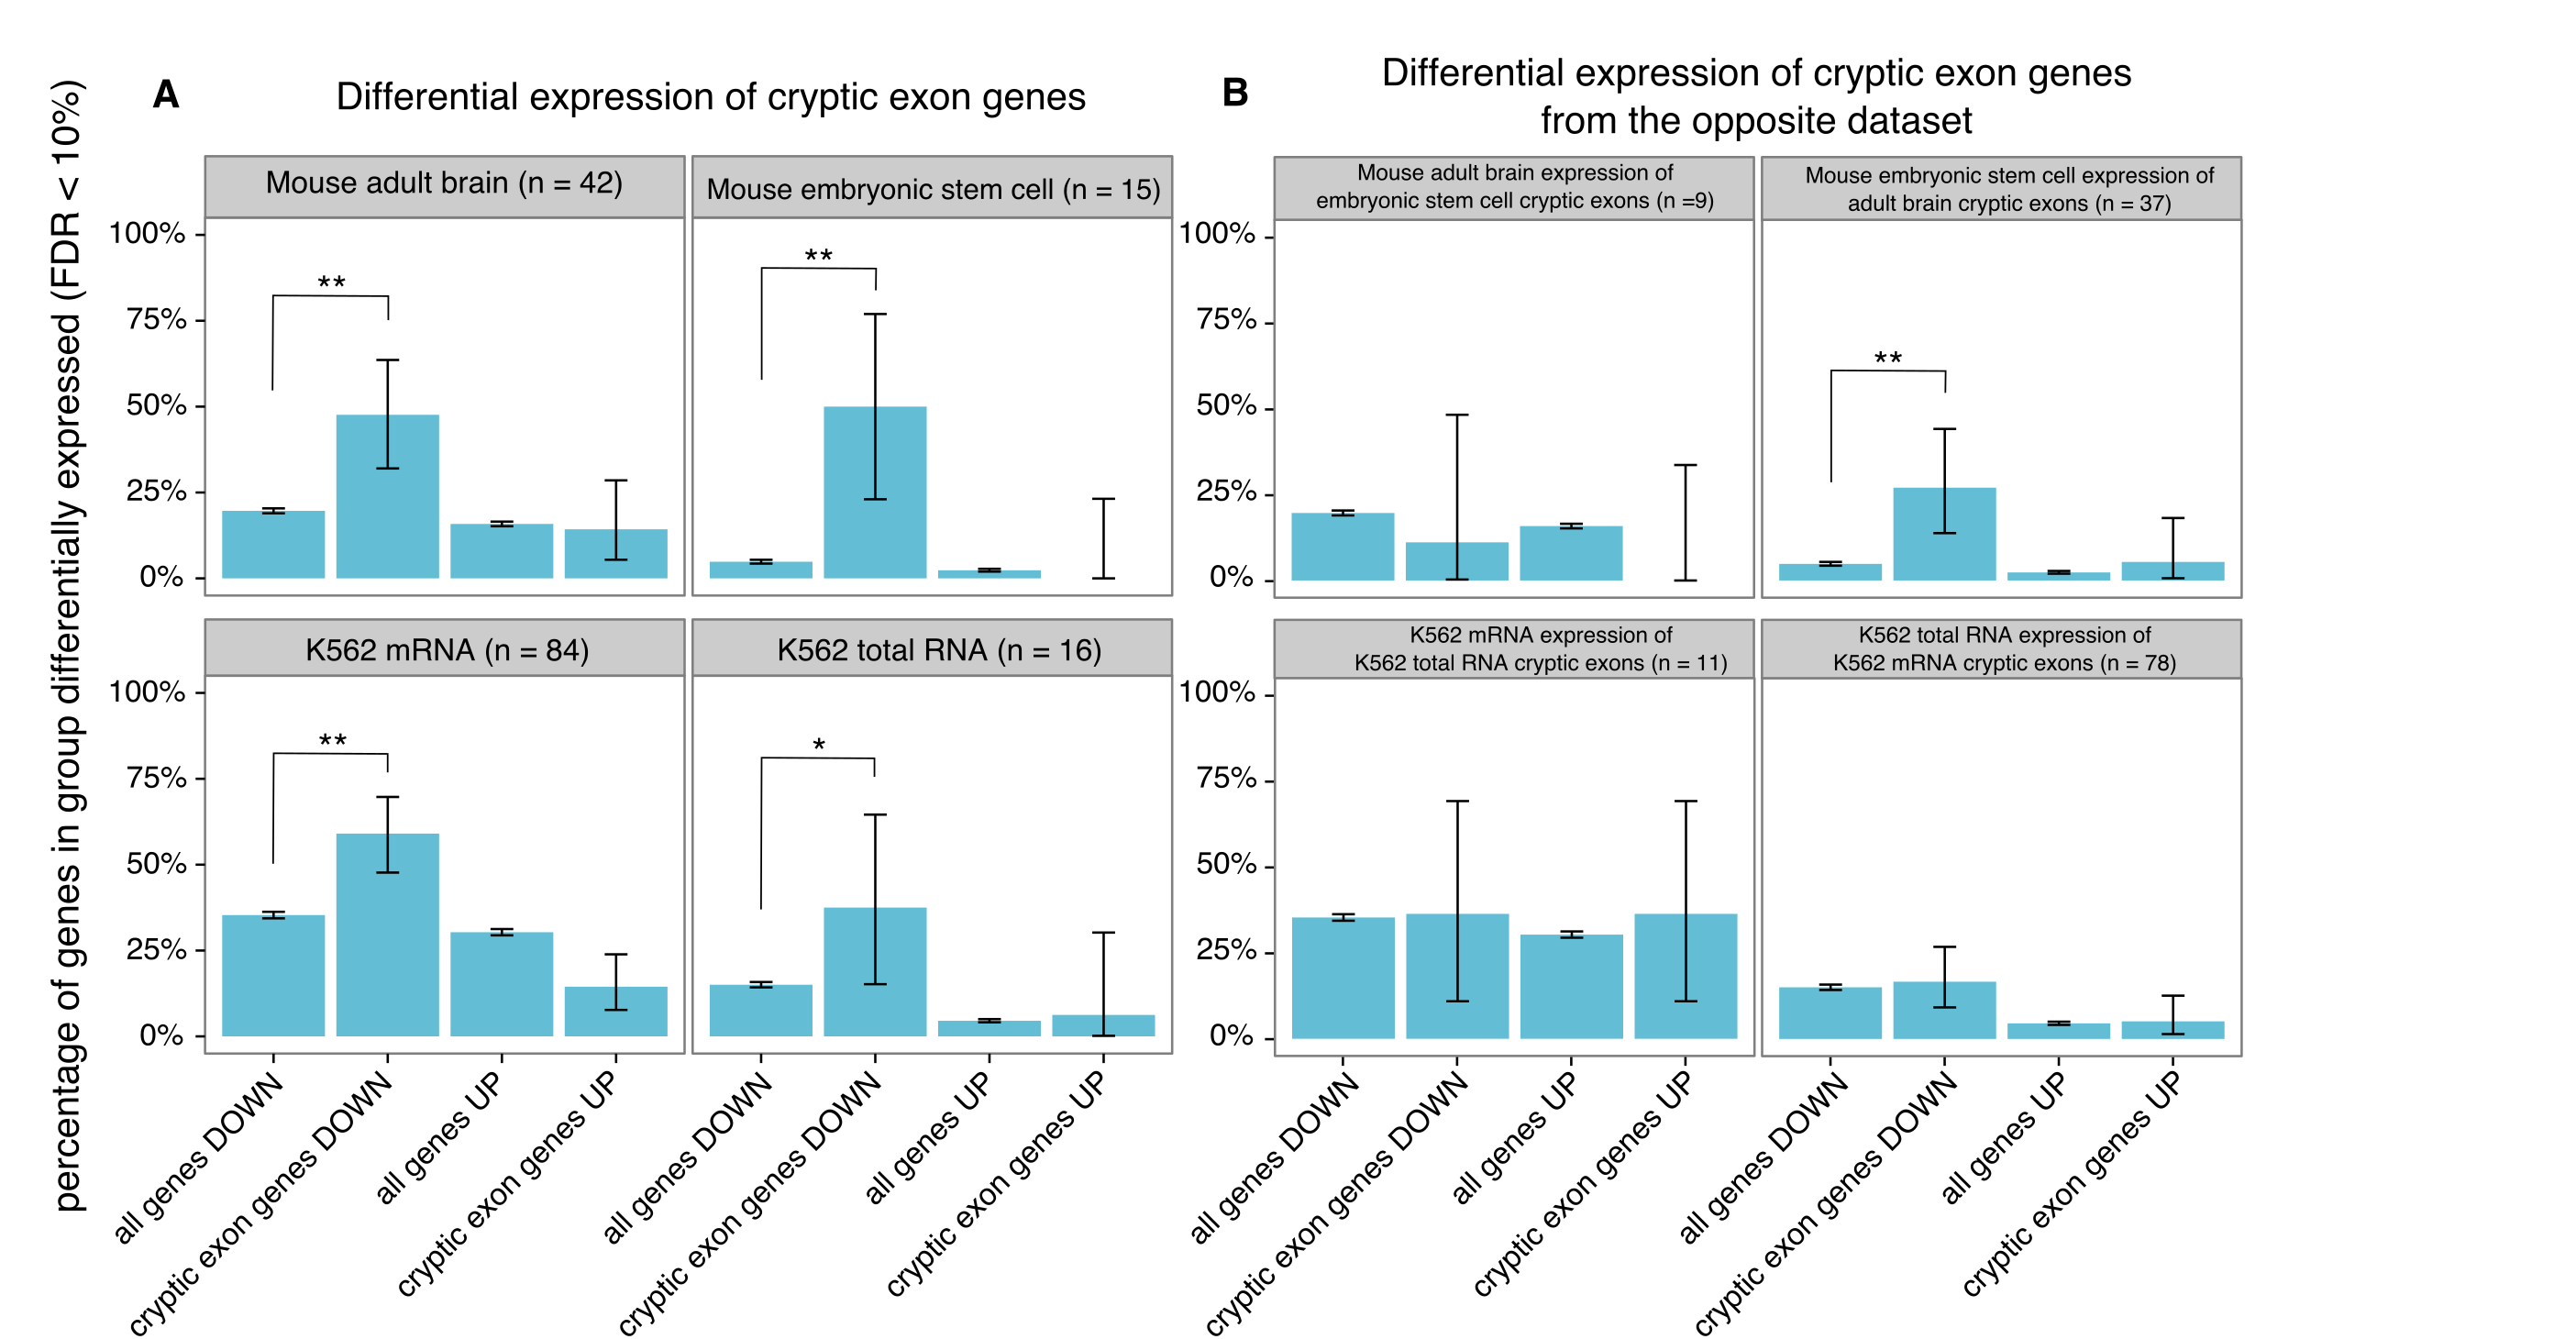
\includegraphics[width=\textwidth, trim = {0.2cm 0 3cm 0}, clip]{Figures/03_cryptic_exons/Figure_5_Gene_Expression.png}
	\caption[Differential expression of cryptic exon genes]{
		\textbf{Differential expression of cryptic exon genes.}
	\textbf{(A)} Significantly differentially expressed genes between TDP-43 depletion and control samples (false discovery rate = 10\%) in datasets 3-6. Comparisons were made between all genes tested with an expression level at or greater than the lowest expressed cryptic exon (``all genes'') and the genes where cryptic exons were discovered (``cryptic exon genes'') with each group divided by direction of change. 
	\textbf{(B)} As above but for cryptic exon genes from the other dataset of the same species. Error bars show 95\% confidence intervals for each proportion. $^* : P < 0.05$, $^{**} : P < 0.001$. All \textit{P}-values adjusted by Bonferroni correction.
}	
	\label{fig:cryptic_expression}
\end{figure}

I then investigated, in datasets 3-6, whether genes containing cryptic exons showed a specific pattern of altered expression. I calculated the proportion of the cryptic exon containing genes in each dataset that were differentially expressed at a FDR of 10\%. This was then compared with the proportion of differential expression of all genes with an expression level at or greater than the lowest expressed cryptic exon found in that dataset. I then plotted the number of differentially expressed genes in each dataset as a proportion of the total, separated by direction. In all four TDP-43 depletion datasets, the cryptic exon containing genes as a group are more likely to be significantly downregulated compared to the genome-wide proportion ($P < 0.001$, hypergeometric test; Fig. \ref{fig:cryptic_expression}A).

Furthermore, I performed the same analysis for each dataset with the cryptic exon containing genes that were only found in the other dataset of the same species (Fig. \ref{fig:cryptic_expression}B). Surprisingly, in the mouse ES cell dataset 6 there was an enrichment of downregulated genes that contain cryptic exons only detectable in the mouse adult brain dataset 5 ($P < 0.001$, hypergeometric test). Visual inspection of these 10 introns in the mouse ES cell data suggests that 7 of them may harbour cryptic exons in the ES cell data that are currently undetectable by the \emph{CryptEx} algorithm.


\subsection{Human cryptic exons are driven by the recognition of strong splice sites that are normally repressed}

\begin{figure}[h!]
	\centering
	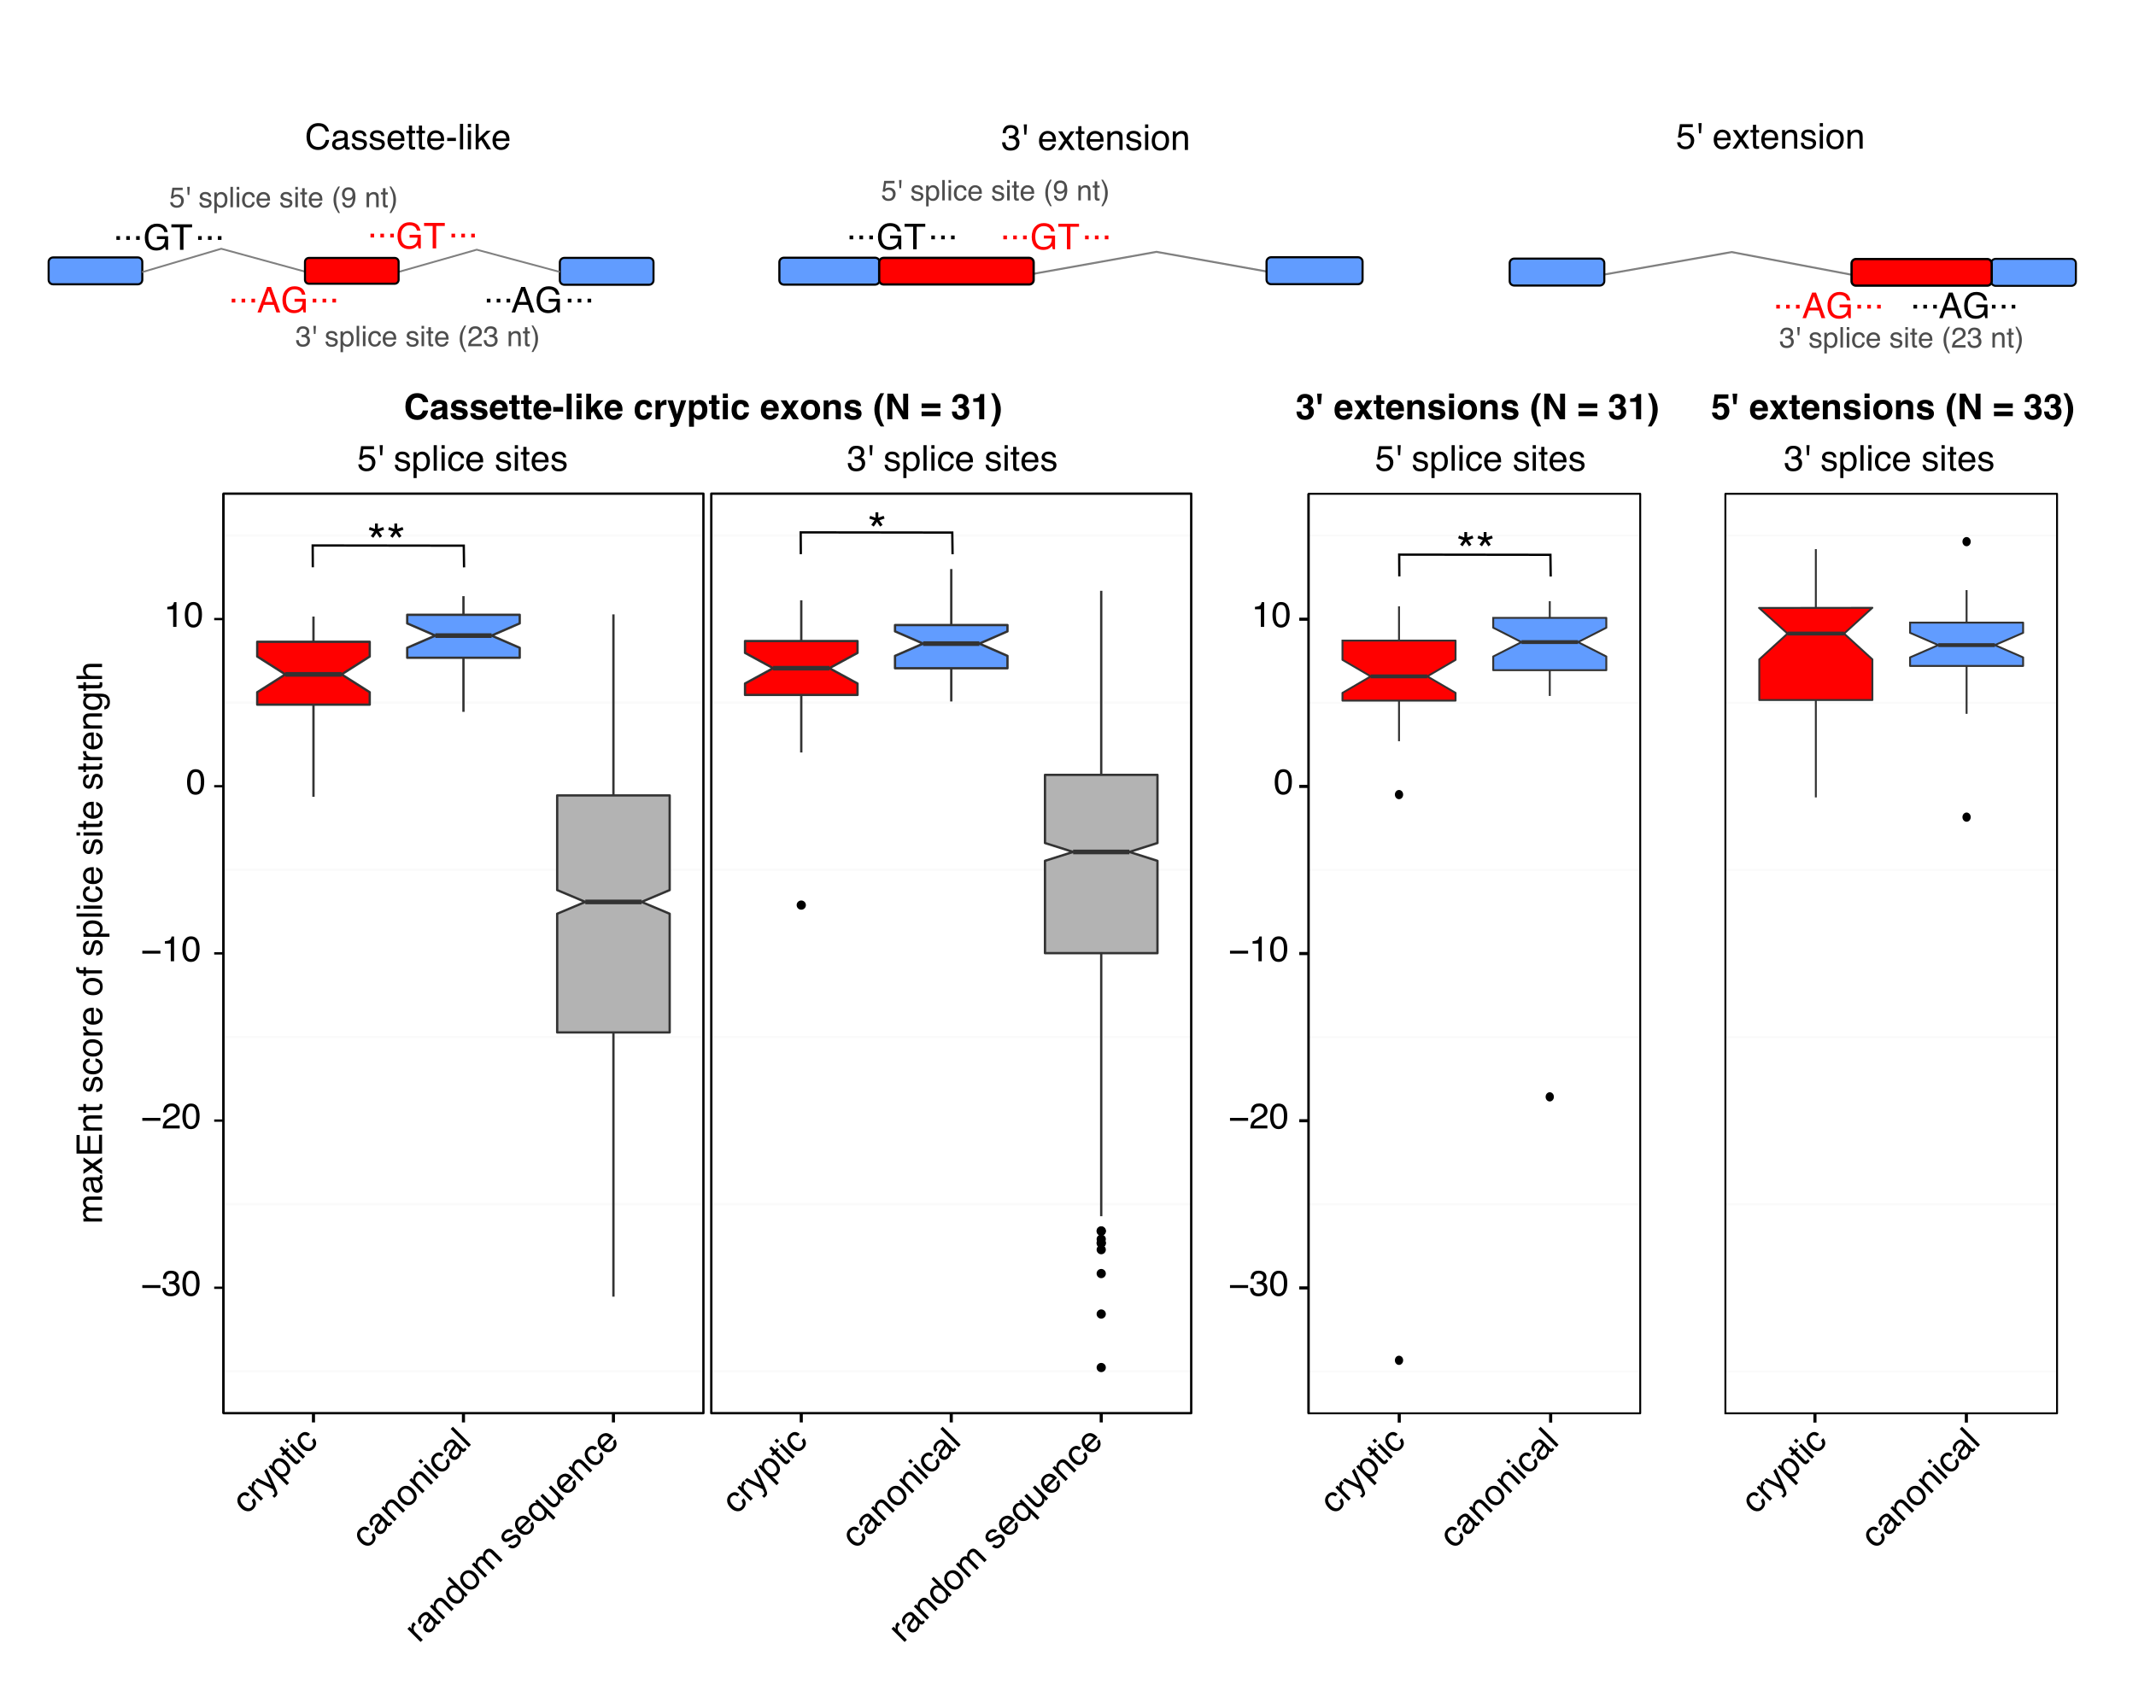
\includegraphics[width=\textwidth]{Figures/03_cryptic_exons/Figure_6_splice_site_scoring.png}
	\caption[Scoring cryptic splice sites against canonical splice sites]{
		\textbf{Scoring cryptic splice sites against canonical splice sites.}
		Cassette-like cryptic exons have 5\'\ and 3\'\ splice sites that are recognised by the spliceosome under TDP-43 depletion. 5\'\ and 3\'\ splice site scores are plotted separately. Cryptic splice sites are shown in red, canonical splice sites are shown in blue. Random sequences with AG or GT consensus are plotted in grey. Cryptic extensions are the result of a cryptic splice site competing with the canonical splice site. 5\'\ extensions result from cryptic 3\'\ splice sites whereas 3\'\ extensions result from cryptic 5\'\ splice sites. Box plots show first quartile, median and third quartile with the notches representing the 95\% confidence interval of the median. Whiskers represent the minimum and maximum values that fall within 1.5 times the interquartile range. Outliers are plotted as black dots. Cryptic splice sites are compared to canonical splice sites with paired t-tests. $^{*}: P < 0.05$, $^{**}: P < 0.001$.
}
	\label{fig:cryptic_scoring}
\end{figure}

Whereas cassette-like cryptic exons appear as separate exons distinct from their surrounding exons, extension events must rely on a switch from a canonical splice site to a newly accessible splice site. I hypothesised that these extension events result from competition between two splice sites upon TDP-43 depletion. This would require the sequence of and around the cryptic splice site to be similarly recognisable to the spliceosome. Using the \emph{MaxEnt} statistical model to score splice sites by comparing their DNA sequences with constitutive observed canonical sequences, I scored the 5\'\ and 3\'\ splice sites of our cryptic exons and compared them with the scores of the surrounding canonical splice sites. The model compares splice sites from annotated exons with decoy splice sites that retain the consensus AG/GT at the 3\'\ or 5\'\ splice site respectively. Therefore I also scored randomly generated sequences which retained the consensus AG/GT positions.  Although the canonical splice sites were on average stronger than their corresponding cryptic splice site ($P < 0.05$, paired t-test), the majority had scores far greater than those from random sequence (Fig. \ref{fig:cryptic_scoring}), suggesting that they are able function as genuine, albeit weaker, splice sites when TDP-43 is depleted.



\subsection{TDP-43 cryptic exons are bound by other RNA binding proteins}

\begin{figure}[h!]
	\centering
	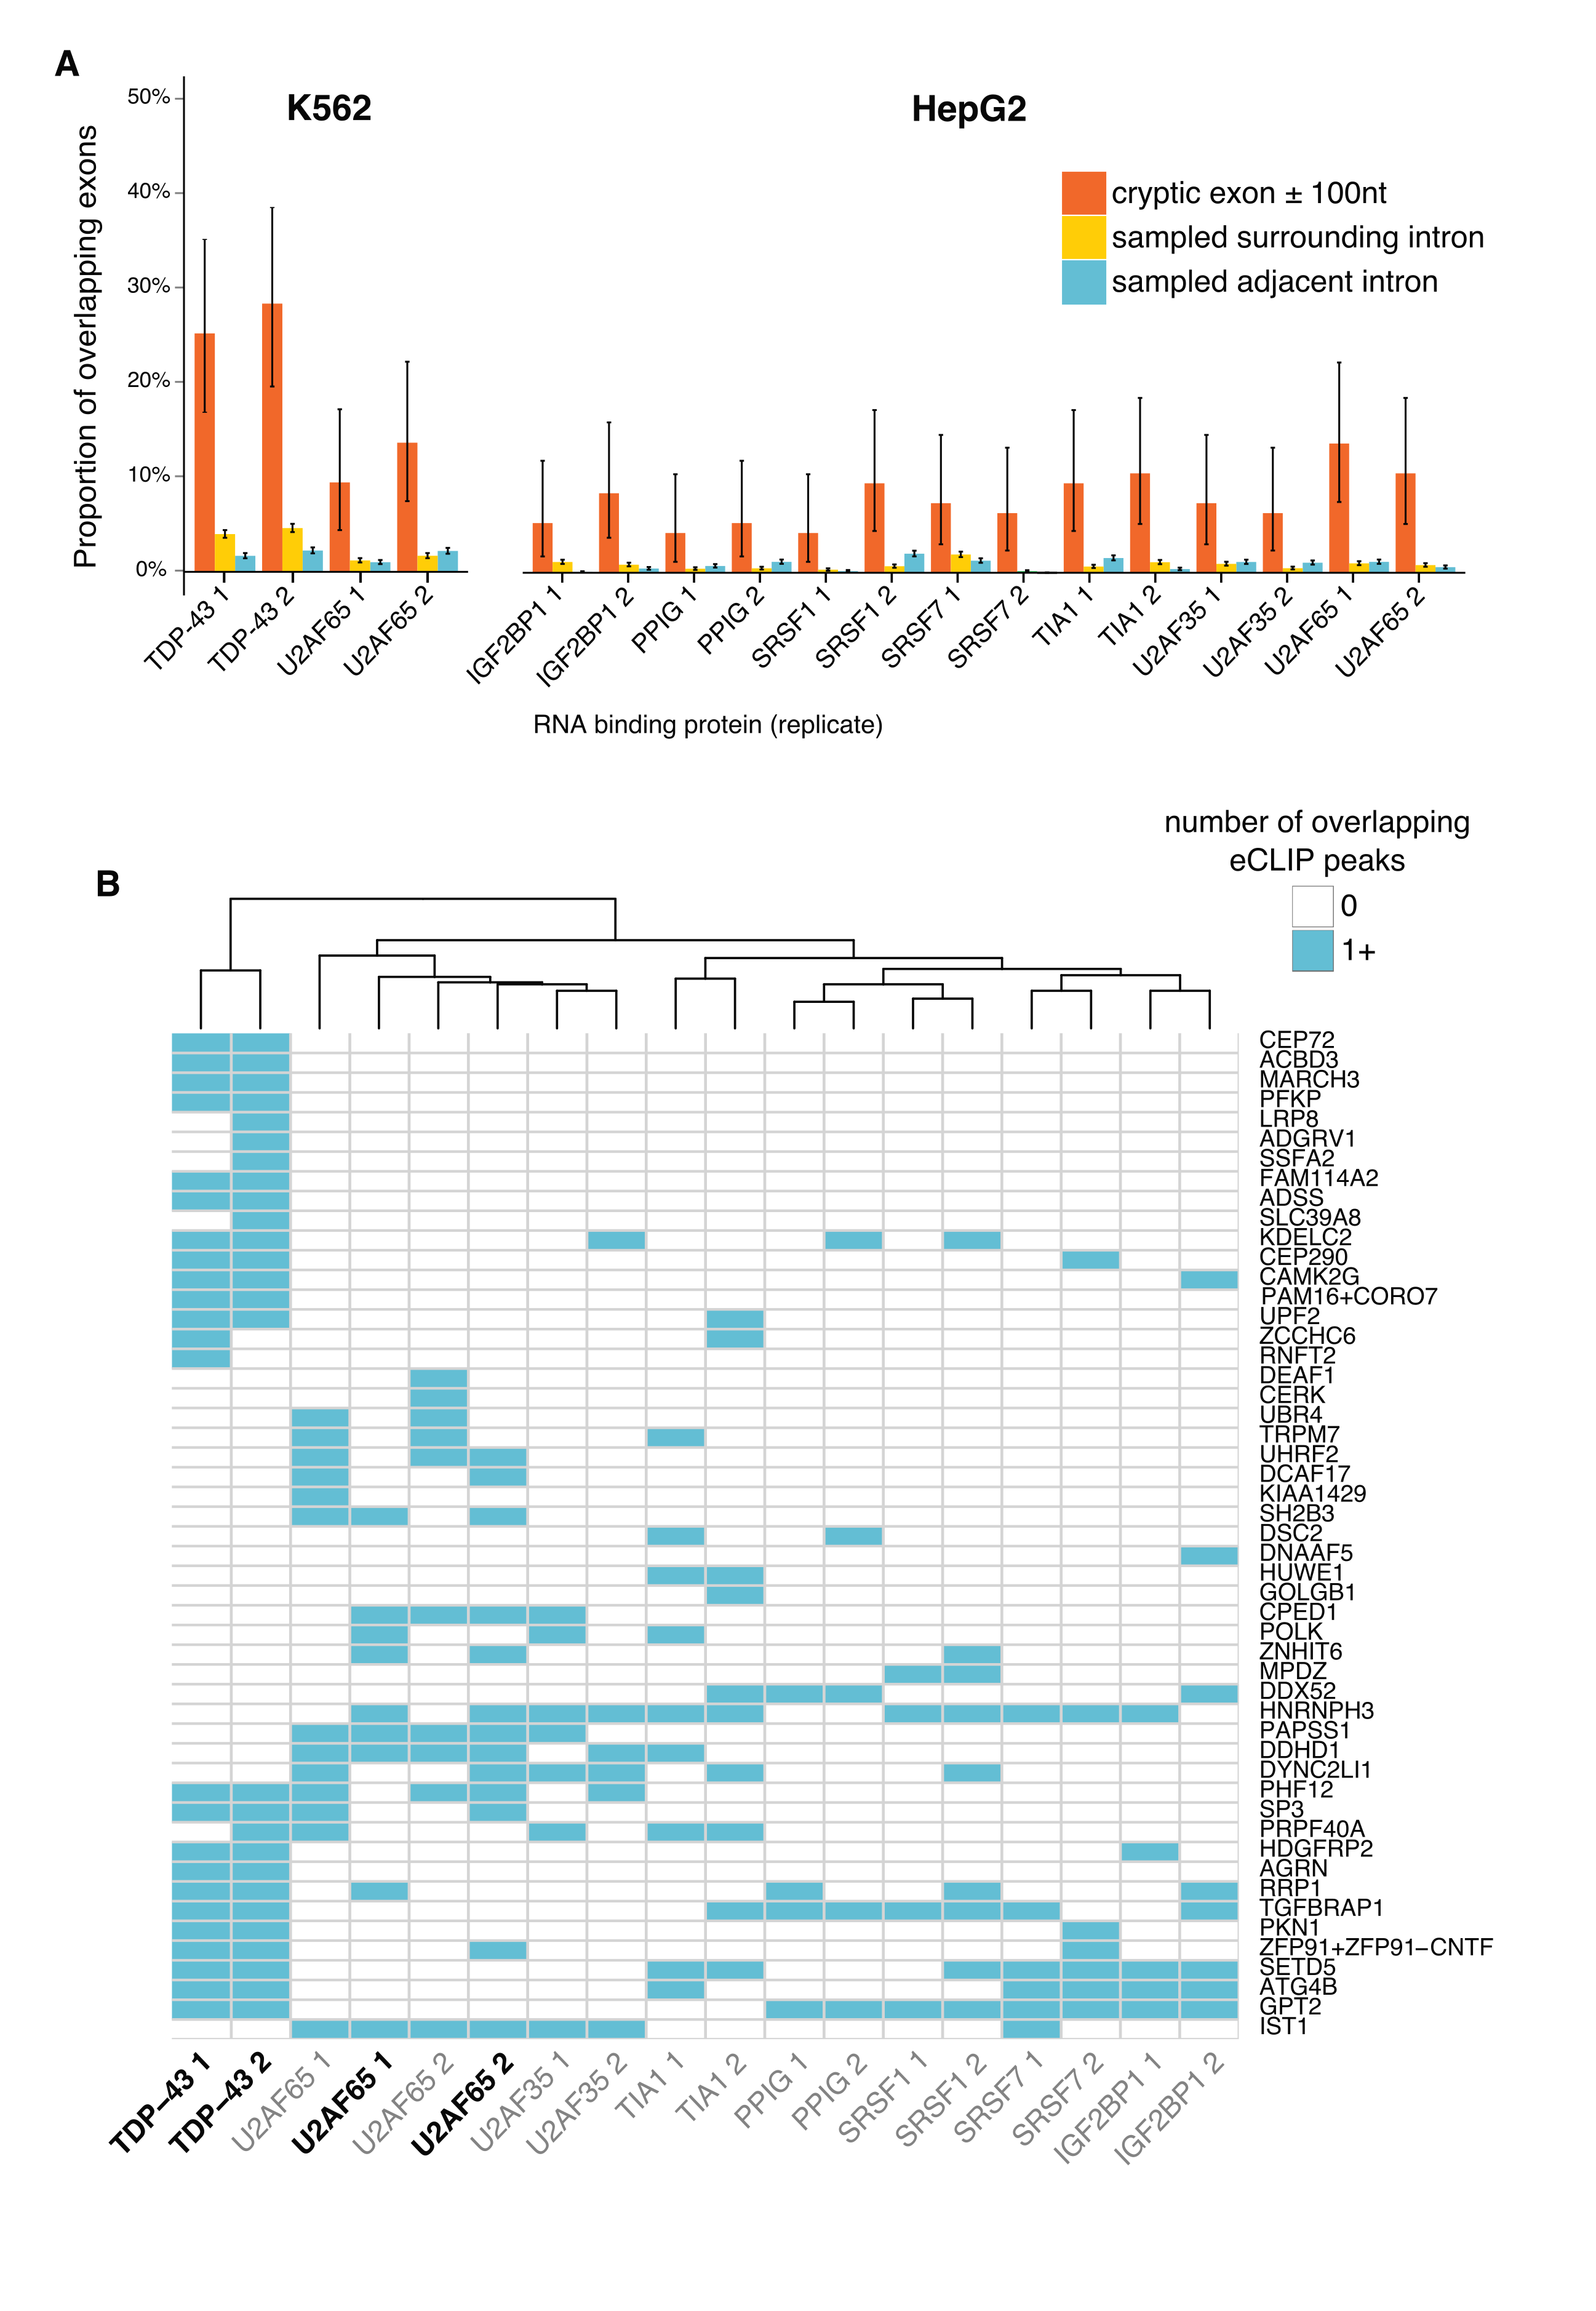
\includegraphics[width=\textwidth]{Figures/03_cryptic_exons/Figure_7_ENCODE_mining.png}
	\caption[Mining of ENCODE eCLIP data in K562 and HepG2 cells]{
		\textbf{Mining of ENCODE eCLIP data in K562 and HepG2 cells.}
	\textbf{(A)} RNA-binding proteins (RBPs) with significant ($P < 0.05$) proportion of overlapping cryptic exons (red) compared to sampled intronic sequence from the same (green) and adjacent introns (blue). 
	\textbf{(B)} Comparison of eCLIP datasets from different RNA binding proteins (columns) showing the overlap with the cryptic exons (rows). RBPs in bold typeface are from K562 cells whereas those in regular typeface are from HepG2 cells.
}
	\label{fig:cryptic_mining}
\end{figure}

Proteomic studies have demonstrated that TDP-43 interacts with a number of RNA-binding proteins (RBPs), including multiple members of the heterologously expressed ribonucleoprotein (hnRNP) family and other splicing factors \citep{Blokhuis2016-hw,Ling2010-sr,Freibaum2010-hw}. The splicing of specific annotated exons has been shown to depend on the interaction of TDP-43 with multiple splicing factors \citep{Mohagheghi2016}.  I hypothesised that some cryptic exons may be included indirectly through a loss of interactions with different RBPs. Van Nostrand and colleagues have performed eCLIP, a higher throughput modification of the iCLIP protocol, on 73 different RBPs including TDP-43 and FUS \citep{Van_Nostrand2016-su}. The experiments were carried out in 2 human cell lines (K562 and HepG2) with 29 of the RBPs being tested in both cell lines. I performed the same overlap analysis between our human cryptic exons and each set of eCLIP peaks, using the same two sets of control sequences as before. Each eCLIP experiment was performed in duplicate. This gives each RBP four possible enrichment results using a proportion test. For each RBP, the highest P-value from the four tests was reported and corrected for multiple testing. Only proteins with a resulting $P < 0.05$ are reported. Unsurprisingly TDP-43 had the highest number of overlapping exons ($p < 10^{-22}$; proportion test), followed by U2AF65, TIA1, SRSF7, U2AF35, PPIG, SRSF1 and IGF2BP1 (Fig. \ref{fig:cryptic_mining}A). Hierarchical clustering was performed on the RBPs. The three largest clusters consist  of TDP-43 alone, the U2 snRNP binding proteins U2AF35 and U2AF65, and a third cluster containing the other proteins (Fig. \ref{fig:cryptic_mining}B). 

\clearpage

\section{Discussion}
I designed an analytical strategy to identify cryptic splicing that takes advantage of biological replicates in RNA sequencing data. I have applied this tool to a set of human and murine TDP-43 depletion datasets, as well as datasets that deplete hnRNP C or FUS. The results are consistent with the previous findings that depletion of TDP-43 or hnRNP C leads to the inclusion of novel cryptic exons in both human and mouse. Although FUS undoubtedly plays an important role in splicing and mRNA stability and shares a number of targets with TDP-43 \citep{Lagier-Tourenne2012}, the low number of cryptic exons observed due to FUS depletion suggests that it does not play a major role in cryptic splicing and is a key point of differentiation with TDP-43.

Further examination of TDP-43 linked exons suggests they tend to possess the necessary UG-rich sequence elements to be bound by TDP-43 and using iCLIP data I observed that a subset of the cryptic exons are shown to be bound by TDP-43 \emph{in vivo}. I went on to investigate the origins of these TDP-43 bound cryptic exons, as has been done for the targets of hnRNP C. I observed that unlike hnRNP C linked cryptic exons, which invariably originate from antisense Alu elements, TDP-43 linked cryptic exons do not originate from any single family of transposable element. Furthermore their sequences show very low species conservation, akin to random intronic sequence, but remarkably they contain splice sites very close in strength to those of their adjacent annotated exons. Differential expression analysis suggests that the bulk of cryptic exon containing genes are significantly downregulated upon TDP-43 depletion. I hypothesize that this is due to nonsense mediated decay of the inclusion transcript, which I predict would occur in over 90\% of cryptic exon containing transcripts. Comparing my human cryptic exons with a proteomic study of TDP-43 depletion in human SH-SY5Y cells \citep{Stalekar2015-qd} showed that protein levels were changed for 3 of the 95 human cryptic exon containing genes. Two, \emph{HUWE1} and \emph{GOLGB1} had protein levels that were 8\% and 31\% of the control cells respectively whereas the third, \emph{HNRNPH3} was found to be 7-fold increased under TDP-43 depletion. Interestingly, the cryptic exon discovered in hnRNP H3 falls upstream of the start codon whereas those found in \emph{HUWE1} and \emph{GOLGB1} are predicted to trigger NMD by inclusion of intronic RNA into the coding sequence (see Supplementary Table 1).  Another gene with cryptic splicing seen in both K562 datasets and in the initial Ling HeLa data, \emph{AGRN}, has been shown to be decreased at the protein level in the cerebrospinal fluid of ALS patients compared to healthy controls and other neurological diseases \citep{Collins2015-xd}. Correct splicing of \emph{AGRN} has shown to be crucial for the formation of the neuromuscular junction \citep{Ruggiu2009-qx}.

My understanding of TDP-43's role in cryptic splicing is that of a safeguard against the inclusion of potentially damaging intronic sequence into transcripts. However, the relationship between the UG-rich sequences and the strong 5\'\ and 3\'\ splice sites and their changes over evolutionary time are unknown as we observed no conserved cryptic exons between human and mouse. 

Using publicly available ENCODE eCLIP data, I identified a number of RNA binding proteins that also bind subsets of human cryptic exons under normal conditions, that is, in the presence of TDP-43.  It is unsurprising that the splicing factors U2AF35 and U2AF65 are enriched as they preferably bind pyrimidine-rich 3\'\ splice site sequences which all cryptic exons appear to possess. That only 10-15\% of cryptic exons show U2AF35/65 binding may be due to competition from TDP-43 in a manner similar to that seen between hnRNP C and U2AF65 \citep{Zarnack2013}. TIA1 is an exciting finding due to its role in the formation of stress granules, which are key regulators of RNA stability \citep{gilks2004stress}. In addition, IGF2BP1 has been reported to be bound to TDP-43 in HEK293T and HeLa cell extracts \citep{Ling2010-sr,Freibaum2010-hw}, whereas SRSF7 was reported as binding to TDP-43 in mouse N2A cells \citep{Blokhuis2016-hw}. None of the observed proteins have been reported to change their protein level in response to TDP-43 depletion \citep{Stalekar2015-qd}.

As the majority of cryptic exons are predicted to lead to nonsense-mediated decay of the inclusion transcript it seems peculiar that we can observe these transcripts at all. I hypothesise that cryptic splicing may be much more widespread than can be observed by RNA sequencing due to the highly efficient nature of nonsense mediated decay. Over half of all cryptic exon genes are significantly downregulated in each dataset (Fig \ref{fig:cryptic_expression}B), suggesting that cryptic exon inclusion may be a key mechanism in the widespread changes in RNA expression that occur upon TDP-43 depletion. This has been explored in hnRNP C, where a large increase in the number and observed inclusion of Alu-derived cryptic exons was seen when both hnRNP C and the nonsense mediated decay-associated protein UPF1 were co-depleted compared to just hnRNP C or UPF1 alone \citep{Attig2016}.

Two genes, \emph{ATG4B} and \emph{GPSM2}, have previously been demonstrated to have cryptic exon inclusion RNA transcripts in ALS patient brain samples, suggesting a role for cryptic splicing in disease \citep{Ling2015}. My analysis also identified a cryptic exon in \emph{ATG4B} in human cells, but not \emph{GPSM2}; however I did not analyse human brain data. By expanding the list of cryptic exons, it will be interesting to explore whether these are also dysregulated in ALS patient brains. However, such analysis may prove challenging owing to the likely small concentrations of RNA originating from diseased cells in brain homogenate and the likelihood of degradation by NMD. Alternate strategies may involve mass spectrometry screens for the subset of cryptic exon containing genes that escape the NMD process, for example because the cryptic exon is in frame. Such proteins may represent useful biomarkers for ALS. 

A complementary bioinformatic method was used increase the number of cryptic exons seen in the original Ling data \citep{Tan2016}. This study extends the cryptic splicing phenomenon to RBM17, another RNA-binding protein, making the very low number of cryptic exons observed in the FUS depletion datasets even more surprising.

Defining cryptic exons by their absence in existing annotation is not a suitable long term strategy. For example, the \textit{SORT1} gene contains an exon normally repressed by TDP-43 and not constitutively included in any tissue \citep{Prudencio2012}. But due to the studies that have documented its existence the "cryptic" exon in \textit{SORT1} is annotated in all transcript databases. There are certainly many examples of annotated exons that are extremely rarely included and may be repressed by splicing factors like TDP-43. Future studies may have to take a more measured approach based on the frequency of inclusion in multiple tissues and conditions to assess whether an exon is truly cryptic or not.


\subsection{Epilogue: Cryptic exons are a widespread phenomenon seen in many RNA-binding proteins}

\begin{figure}[h!]
	\centering
	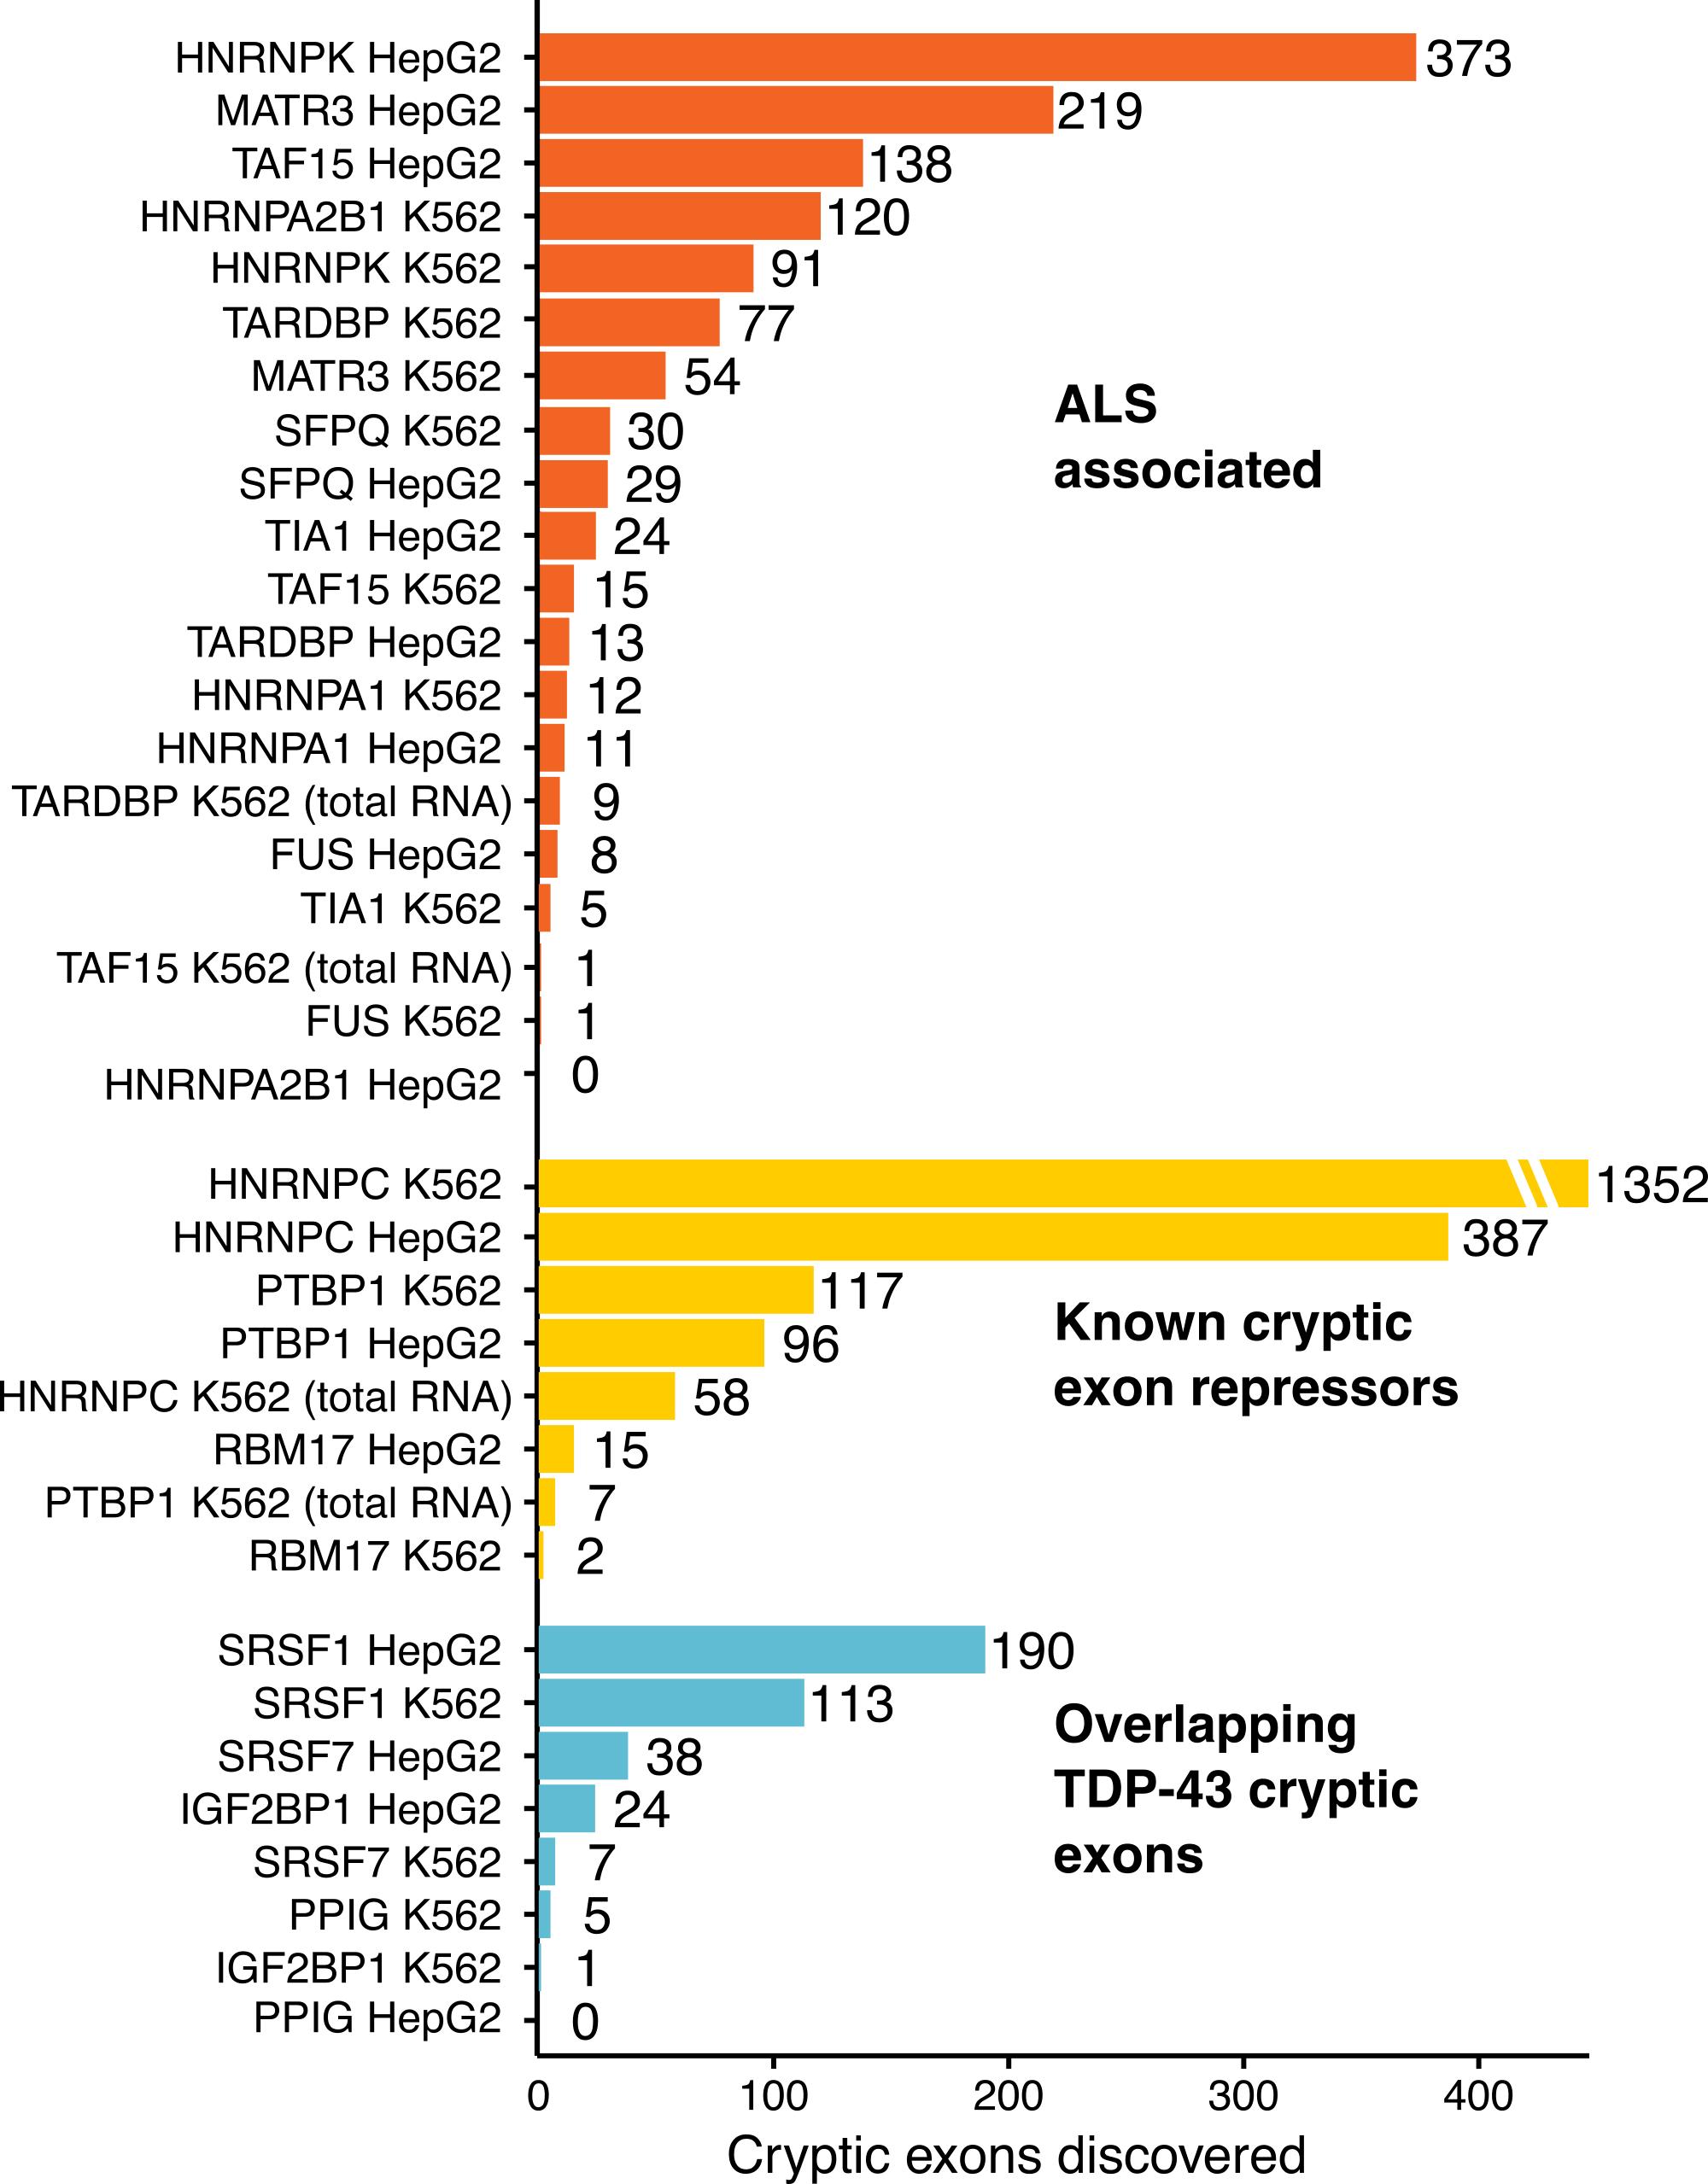
\includegraphics[width=12cm]{Figures/03_cryptic_exons/all_ENCODE_cryptex_counts.png}
	\caption[Cryptic exons found in different ENCODE shRNA knockdowns]{\textbf{Cryptic exons found in different ENCODE shRNA knockdowns}}
	\label{fig:cryptic_counts}
\end{figure}

Following completion and publication of this work, I downloaded a selection of shRNA knockdowns of RNA-binding proteins from the ENCODE portal. 
This included every available protein linked to ALS, including TIA1 and SFPQ, recently shown to harbour rare disease-causing mutations \citep{Mackenzie2017,Thomas-Jinu2017}.
In addition I downloaded knockdowns of hnRNP K, a splicing factor which interacts with TDP-43 \citep{Freibaum2010-hw} and plays a role in regulating TDP-43 aggregation \citep{Moujalled2015}.
All data was aligned and run through the \textit{Cryptex} pipeline for cryptic exon discovery. Cryptic exon abundances were compared between the knockdowns and their scrambled shRNA controls.

hnRNP K knockdown in HepG2 and K562 cells lead to the inclusion of 373 and 91 cryptic exons respectively (Fig \ref{fig:cryptic_counts}), the largest effect seen in this set of proteins.
MATR3 knockdown led to 219 and 54 cryptic exons. MATR3 has now been linked to cryptic splicing through binding within LINE elements \citep{Attig2018}.
Perhaps most surprising is the finding of 138 and 15 cryptic exons being included in the knockdown of TAF15 in HepG2 cells and K562 cells respectively. 
TAF15 is closely related to FUS, in which I only observe 8 and 1 cryptic exons.
This suggests diverging splicing functions between TAF15 and FUS, despite the two proteins binding similar motifs and overlapping RNA targets \citep{Kapeli2016}.
As a comparison I downloaded data from proteins linked to cryptic splicing in other papers such as PTBP1 and RBM17 \citep{Ling2016, Tan2016}, as well as the previously discussed HNRNPC. 
Knockdown of either hnRNP C or PTBP1 leads to a robust number of cryptic exons in both cell types.
Comparatively few events are seen in RBM17, despite 1475 genes being previously observed to harbour cryptic splicing changes in an \textit{Rbm17} knockout mouse \citep{Tan2016}.
In addition I included the proteins seen to be enriched in eCLIP binding to TDP-43 cryptic exons.
Surprisingly nearly all proteins assessed show evidence of cryptic splicing upon their knockdown, with SRSF1 knockdown having the most.
Together this shows that repression of cryptic splice sites is probably a more general function of RNA-binding proteins than previously realised. 
This makes the seeming lack of cryptic splicing seen in FUS knockdown all the more intriguing.
% caveats


\section{Summary}
In this project I replicate and confirm the presence of cryptic exons after TDP-43 depletion and show they have a negative impact on the genes they reside in, leading to decreased expression levels.  I have extended the scale and understanding of cryptic exons and their relation to TDP-43. In addition, I have demonstrated a key difference between FUS and other ALS-associated RNA-binding proteins. Further work is warranted to determine the relevance of cryptic exons to ALS and FTD pathogenesis.


